\documentclass[11pt]{article}
% alternative fonts: 
% times, mathptmx, mathpazo, newcent, bookman
% xref http://www.ce.cmu.edu/~kijoo/latex2pdf.pdf
\usepackage{newcent}
\usepackage{fullpage}
\usepackage{fancyvrb}
\usepackage[authoryear]{natbib}
\usepackage[pdftex]{graphicx}
\usepackage[backref,colorlinks]{hyperref}


% Typography.
\newcommand{\ccode}[1]{{\small\texttt{#1}}}
\newcommand{\emcode}[1]{{\small\bfseries\texttt{#1}}}
\newcommand{\prog}[1]{\small\texttt{#1}}
\newcommand{\eslmod}[1]{{\smaller\bfseries\texttt{#1}}}
\newcommand{\eslfunc}[1]{\hyperlink{man:#1}{{\small\texttt{#1}}}}

% Eliminate the ones below someday. 
\newcommand{\cmacro}[1]{\texttt{#1}}
\newcommand{\cvar}[1]{\texttt{#1}}
\newcommand{\cvartype}[1]{\texttt{#1}}
\newcommand{\cstruct}[1]{\texttt{#1}}
\newcommand{\cfunc}[1]{\texttt{#1}}
\newcommand{\cfile}[1]{\texttt{#1}}

\def\argmax{\mathop{\mathrm{argmax}}\limits}
\def\argmin{\mathop{\mathrm{argmin}}\limits}

\DefineVerbatimEnvironment{cchunk}{Verbatim}{fontsize=\scriptsize,xleftmargin=2.0\parindent}%

% Description-like environment for documenting functions/APIs.
% puts the description label in a minipage with a large hanging
% indent.
% Good christ this took a long time to develop.
% hanging indent trick stolen from Peter Wilson's hanging.sty @CTAN
% minipage allows multi-line label, and puts item on next line.
% customized list inspired by Kopka/Daly _Guide to LaTeX_ p.213
% SRE, Wed Dec 27 11:37:18 2000
%
\newenvironment{sreapi}{%
     \begin{list}{}{%
       \renewcommand{\makelabel}[1]{%
         \begin{minipage}{\textwidth}%
           \hangindent10em\hangafter1\noindent%
           {\bfseries\texttt{##1}\vspace{0.8em}}%
         \end{minipage}%
     }}}%
     {\end{list}}


% Description-like environment for producing lists like:
%
%     label  stuff, stuff, stuff
%
%    label2  more stuff, more stuff,
%            more stuff.
% \begin{sreitems}{Longest label} \item[label] stuff, ... \end{sreitems}
% SRE, Wed Dec 27 11:59:43 2000
%
\newenvironment{sreitems}[1]{%
     \begin{list}{}{%
       \settowidth{\labelwidth}{#1}%
       \setlength{\leftmargin}{\labelwidth}%
       \addtolength{\leftmargin}{\labelsep}%
       }}
     {\end{list}}


\begin{document}

\begin{titlepage}
{\Large

\vspace*{\fill}

\noindent
{\Huge{Easel}} \\ 
\rule[2pt]{\textwidth}{1pt} \\
\hspace*{\fill} {\large {A library of C functions for
    biosequence analysis} \\ }

\vspace*{\fill}

\begin{center}
\url{http://selab.janelia.org/easel/}\\
Version 0.1; May 2007 \\ 

\vspace*{\fill}

Sean Eddy\\
HHMI Janelia Farm Research Campus\\
19700 Helix Drive\\
Ashburn VA 20147\\
\url{http://selab.janelia.org/}\\
\end{center}

\vspace*{\fill}
}
\end{titlepage}

\vspace*{\fill}

\noindent 
Copyright (C) 2004-2005 HHMI/Washington University School of
Medicine.\\

\vspace{1.5em}
\noindent 
The Easel library, including both the software and its documentation,
is licensed and freely distributed under the Creative Commons
Attribution License.  To view a copy of this license, visit
\url{http://creativecommons.org/licenses/by/2.0/} or send a letter to
Creative Commons, 559 Nathan Abbott Way, Stanford, California 94305,
USA.



\newpage
\tableofcontents

\newpage
\section{Introduction}
\section{Overview of modules}
\begin{tabular}{llll}\hline
\textbf{Module} & \textbf{Description}       & \textbf{Requires} & \textbf{Augmentation(s)}\\\hline
  \multicolumn{4}{c}{\textbf{Core module}}\\
easel           & Framework for using Easel         &  -     & \\
  \multicolumn{4}{c}{\textbf{Foundation modules}}\\
alphabet        & Digitized biosequence alphabets   & easel  & \\
dmatrix         & Matrix algebra                    & easel  & \\ 
getopts         & Command line parsing              & easel  & \\
keyhash         & Keyword hashing                   & easel  & \\
msa             & Multiple sequence alignment i/o   & easel  & keyhash \\
parse           & Token-based file parsing          & easel  & \\
random          & Random number generator           & easel  & \\
regexp          & Regular expression matching       & easel  & \\
sqio            & Sequence file i/o                 & easel  & alphabet, msa\\
stack           & Pushdown stacks                   & easel  & \\
vectorops       & Vector operations                 & easel  & \\\hline
  \multicolumn{4}{c}{\textbf{Derived modules}}\\
bioparse\_paml  & PAML rate matrix datafiles        & easel dmatrix parse & \\
dirichlet       & Dirichlet densities               & easel gamma random & \\ 
gamma           & Gamma densities                   & easel random & \\
ratematrix      & Evolutionary rate matrices        & easel dmatrix vectorops & \\
wuss            & RNA structure annotation          & easel stack    & \\\hline
  \multicolumn{4}{c}{\textbf{Optional library interfaces}}\\
interface\_gsl    & GNU Scientific Library          & easel dmatrix & \\
interface\_lapack & LAPACK linear algebra library   & easel dmatrix & \\\hline
\end{tabular}



\section{Overview of data structures}

\begin{tabular}{lll}\hline
\textbf{Object}          & \textbf{Implemented in} & \textbf{Description}\\\hline
\ccode{ESL\_ALPHABET}    & \cfile{alphabet}        & Digitized sequence alphabet\\
\ccode{ESL\_DMATRIX}     & \cfile{dmatrix}         & 2D double-precision matrix for linear algebra \\
\ccode{ESL\_FILEPARSER}  & \cfile{parse}           & Simple token-based input file parser\\
\ccode{ESL\_GETOPTS}     & \cfile{getopts}         & Application configuration state\\
\ccode{ESL\_KEYHASH}     & \cfile{keyhash}         & Keyword hash table\\
\ccode{ESL\_MSA}         & \cfile{msa}             & Multiple sequence alignment\\
\ccode{ESL\_MSAFILE}     & \cfile{msa}             & Multiple sequence alignment file parser\\
\ccode{ESL\_PERMUTATION} & \cfile{dmatrix}         & Permutation matrix used in linear algebra\\
\ccode{ESL\_RANDOMNESS}  & \cfile{random}          & Random number generator\\
\ccode{ESL\_REGEXP}      & \cfile{regexp}          & Regular expression pattern-matching machine\\
\ccode{ESL\_SEQFILE}     & \cfile{sqio}            & Biosequence file parser (unaligned)\\
\ccode{ESL\_SQ}          & \cfile{sqio}            & DNA/RNA/protein sequence data\\
\ccode{ESL\_STACK}       & \cfile{stack}           & Pushdown stack\\\hline
\end{tabular}

\section{Module design}

Easel is designed to be used in two different ways: as a C library
(\ccode{libeasel.a}) in the usual C way, or by grabbing individual
source files without the rest of the library.

The ability to borrow individual files from Easel makes it different
from many other C libraries. For example, to get Easel's sequence file
i/o API, for example, you just take the sqio module (the C source
\ccode{esl\_sqio.c} and the header \ccode{esl\_sqio.h}), plus the
obligatory Easel core (\ccode{easel.c} and \ccode{easel.h}). Most of
Easel's modules can stand alone in this way (the \emph{base}
modules). Only a few are dependent on other modules (the
\emph{derived} modules), though even these can be used just by
bringing along the modules they depend on.

There are a couple of reasons to provide standalone capability. One
reason came from teaching a computational molecular biology
course. For homework programming assignments, I wanted to provide
students with simple .c files with well-documented APIs for routine
things like sequence i/o. This was to give them a head start, save
them from implementing boring things, and let them concentrate on
learning algorithms. But at the same time, I wanted them to be able to
see where the functionality was coming from, and to study the .c files
if they wanted, rather than treating the library as a black box -- so
I wanted to give them a few .c files at a time, not a library.

A second reason comes from my frustration with C libraries and code
reuse in bioinformatics in general. If I want to take a single routine
from someone's library (say, gods help us, the NCBI Toolkit), it's
common that that routine has dependencies, and the dependencies have
dependencies, and pretty soon I'm dragging the whole damned library in
just to have access to the routine I wanted. I don't mind that in
standard, widely installed system libraries, but if I'm making a
robustly distributable bioinformatics application, I need to include
in my package all my nonstandard dependencies -- and I really don't
want to have to distribute the entire GNU Scientific Library just to
pick up two GSL functions, all of LAPACK to get one numerical routine,
and the whole NCBI Toolkit to pick up one Toolkit routine.

Thus, Easel is very strictly modular in design. You never need the
entire Easel library to use any one aspect of Easel's
functionality. Most often, you need only the module you're interested
in, plus the core easel module.

To facilitate code reuse, Easel is licensed under a permissive open
source license (the Creative Commons Attribution License) that allows
you to freely modify and redistribute the code.

In the end, some of my original intent of providing simple
implementations as teaching examples has been lost. Rather than
providing two implementations (my intended simple teaching example and
a full-strength production example), Easel code is all production
code. But the modularity remains, and it seems to be useful in other
respects.  Modular design is just a Good Thing in general.  Easel
modules can be unit-tested in absence of the rest of the library.
And, though this remains to be seen, it should be easy for other
people to contribute modules and extend Easel, and it should be easy
for people to borrow and reuse Easel code.

\section{The ``augmentation'' concept}

The trouble with enforcing strict modular design is that while
\emph{you} (the application writer) can take advantage of any or all
of Easel's functionality as you wish, \emph{Easel} can't. An Easel
module, by design, is as isolated as possible from all other Easel
modules. It shouldn't use any functionality other than the essentials
in the core \eslmod{easel} module. But what if module X would benefit
from the cool features of module Y -- for instance, what if we want
the \eslmod{sqio} sequence i/o module to have access to the fast file
indexing capabilities of the \eslmod{ssi} module?  Start down this
road, and pretty soon the library is full of dependencies, the modular
design collapses, and we're back to a standard all-or-none C library.

Easel introduces a concept called \emph{augmentation}. The base
functionality of many Easel modules can be optionally \emph{augmented}
by one or more other Easel modules. An augmentation confers optional
powers on a module beyond its default standalone behavior.

Sometimes, an augmentation adds new functions to a module's API.  For
example, \eslmod{alphabet} augmentation of the sequence i/o module
\eslmod{sqio} adds a function to the \eslmod{sqio} API for digitizing
a sequence.

Sometimes, an augmentation extends or generalizes the scope of one or
more functions in the API. For instance, augmenting the \eslmod{sqio}
module with \eslmod{msa} gives the ability to read alignment files as
if they were sequential, unaligned sequence databases through
\eslmod{sqio}'s existing API.

And sometimes, an augmentation invisibly makes existing functions
faster or more memory-efficient, without adding any new functionality
per se.  For example, \eslmod{msa} can be augmented by
\eslmod{keyhash}, which makes the \eslmod{msa} module capable of
handling much larger alignments more efficiently than it does by
default, because \eslmod{keyhash} gives it the ability to use fast
hashing methods in its parsers.

When Easel is installed as a library, all modules are fully
augmented. This is done when the library is compiled. The
\ccode{configure} script automatically enables all augmentations when
it sets up the \ccode{easel.h} header, before compiling and installing
the library.

When you borrow an individual module from Easel, you choose whether to
borrow any modules that augment it. To activate an augmentation, you
not only have to compile and link the C code for the extra module
(obviously), you also edit a line in the \ccode{easel.h} header file
before compilation. There is a section at the top of \ccode{easel.h}
that declares which augmentations are to be enabled. You
\ccode{\#define} the appropriate flag for your augmentation to
activate it; for instance, to augment with \eslmod{ssi}, you make sure
\ccode{easel.h} has a line \ccode{\#define eslAUGMENT\_SSI} in place
of \ccode{\#undef eslAUGMENT\_SSI}.

Documentation for modules and their functions always distinguishes
between default functionality and augmented functionality.

\section{Function naming conventions in Easel}

\subsection{Object creation, initialization, destruction}

Most of Easel's objects are allocated on the heap; that is, accessed
exclusively via pointers. Less often, routines may allow an object to
be allocated on the stack.

\begin{sreitems}{\ccode{Create,Destroy}}
\item [\ccode{Create,Destroy}] 
  \ccode{esl\_foo\_Create()} allocates and initializes a new \ccode{ESL\_FOO}
  object, returning a pointer to the new
  object. The \ccode{Create()} function is passed any necessary
  initialization or size information in its arguments.
  \ccode{esl\_foo\_Destroy(obj)} frees all the memory associated
  with a \ccode{ESL\_FOO} object,  given a pointer to the object,
  and returns \ccode{ESL\_OK}. Example:

\begin{cchunk}
ESL_SQ *sq;

sq = esl_sq_Create();
esl_sq_Destroy(sq);
\end{cchunk}
  
\item [\ccode{Open,Close}] 
  Same as \ccode{Create()} and \ccode{Destroy()}, but specifically for
  objects associated with input/output streams. Example:

\begin{cchunk}
char        *seqfile = ``foo.seq'';
ESL_SIO     *sqfp;

sqfp = esl_sio_Open(seqfile);
esl_sio_Close(sqfp);
\end{cchunk}


\item [\ccode{Inflate,Deflate}]
  \ccode{esl\_foo\_Inflate(\&obj)} takes a pointer to the ``shell'' of an
  \ccode{ESL\_FOO} object that has been allocated on the stack, and
  allocates and initializes all the internals of it. The
  \ccode{Inflate()} function is passed any necessary initialization or
  size information in its arguments.  \ccode{esl\_foo\_Deflate(\&obj)}
  frees all the internal memory associated with a \ccode{ESL\_FOO} object,
  given a pointer to the object, but the object shell is left alone.
  The only difference between \ccode{Create,Destroy} and
  \ccode{Inflate,Deflate} is whether the object shell itself is to be
  allocated, or not. Example:

\begin{cchunk}
ESL_SQ  sq;

esl_sq_Inflate(&sq);
esl_sq_Deflate(&sq);
\end{cchunk}



\item [\ccode{Expand,Squeeze}]
   These deal with objects whose contents are not necessarily of a
   fixed size, but can grow and require reallocation of internal data
   fields. A function \ccode{esl\_foo\_Expand()} reallocates an
   \ccode{ESL\_FOO} object to a larger size. Usually, reallocation
   works by doubling the previous allocation. The redoubling strategy
   can result in a fair amount of unused memory overhead (up to
   50\%). A function \ccode{esl\_foo\_Squeeze()} takes a fully-grown
   object and optimizes its memory usage, recovering this wastage
   overhead, on the assumption that no more reallocation will be
   done.



\item [\ccode{Reuse}] 
   \ccode{esl\_foo\_Reuse(obj)} reinitializes an object exactly as a
   \ccode{Create} or \ccode{Inflate} function would initialize it, \emph{without}
   allocating new memory; it reuses memory that has
   already been allocated when the object was originally created or
   inflated. For some objects that are used sequentially (like,
   sequences), reusing one object saves malloc()'s compared to
   lots of Create/Destroy calls. A \ccode{Reuse} function does not
   care whether the object was originally created by a \ccode{Create}
   or a \ccode{Inflate} call. Example:

\begin{cchunk}
ESL_SQ *sq;

sq = esl_sq_Create();
  /* read a sequence into the sq object, have fun with it */

esl_sq_Reuse(sq);
  /* read a second sequence into it */

esl_sq_Destroy(sq);
\end{cchunk}

\end{sreitems}

\subsection{Other common object manipulation functions}

\begin{sreitems}{\ccode{\_Copy(src, dest)}}

\item[\ccode{\_Copy(src, dest)}]
Copies \ccode{src} object into \ccode{dest}, where the caller has
already created the empty \ccode{dest} object. Returns \ccode{ESL\_OK}
on success; throws \ccode{ESL\_EINCOMPAT} if the objects are not
compatible (for example, two matrices that are not the same size).

The order of the arguments is always \ccode{src} $\rightarrow$
\ccode{dest} (unlike the C library's \ccode{strcpy()} convention, which
is the opposite order).

\item[\ccode{\_Duplicate(obj)}] 

Creates and returns a pointer to a duplicate of \ccode{obj}.
Equivalent to (and is a shortcut for) \ccode{dest = \_Create();
\_Copy(src, dest)}. Caller is responsible for free'ing the duplicate
object, just as if it had been \ccode{\_Create}'d. Throws NULL if
allocation fails.

\item[\ccode{\_Set*(obj, value...)}]

Initializes value(s) in \ccode{obj} to \ccode{value}. Special cases of
\ccode{\_Set*} functions may exist, like \ccode{\_SetZero} (set to
zero(s)), or \ccode{esl\_dmatrix\_SetIdentity} (set a dmatrix to an
identity matrix).

\end{sreitems}


\section{Discipline of writing Easel modules}


\subsection{API}

\begin{enumerate}
\item Exposed function names obey Easel conventions.

\item All \ccode{ret\_*} pointers for retrieving info from 
      a function are implemented as optional.

\item On any error (returned or thrown), a function releases any
      memory it has allocated, and all \ccode{ret\_*} pointers are
      \ccode{NULL} or 0, depending on their type.

\item Any function that calls another Easel function must 
      catch any thrown errors. Within Easel, we
      can't assume that the error handler is set to be a fatal
      one.
\end{enumerate}


\subsection{Documentation}

\begin{enumerate}
\item Documentation in .tex files is written to application developers
      (and me); documentation in .c comments is written to Easel
      developers (and me).

\item Every module has a .tex file documenting the module and its API,
      and (if it makes sense) also the particular implementation.

\item Every function exposed to the API can be autodocumented (comment
      header can be converted to \LaTeX) with
      \ccode{autodoc\_functions}, in order to produce appendices
      summarizing the complete Easel function set.
\end{enumerate}


\subsection{Testing}

\begin{enumerate}

\item Every module has a test driver which exercises the API in some
      simple way (and, in the process, provides a ``hello world''
      level example of using the module).

\end{enumerate}











\vspace*{\fill}
\begin{quote}
\emph{Lack of skill dictates economy of style.} \hspace{3em} -- Joey Ramone
\end{quote}     


\newpage
\section{The easel (esl) module: error handling and other fundamentals}
The easel (esl) module implements a small set of functionality shared
by all the modules: notably, the error-handling system.

\subsection{Error handling}

Easel is intended for use in applications ranging from quick \& dirty
one-off command line applications to complex graphical user interfaces
and parallel systems. Simple and complex applications have different
views of how errors and exceptions should be handled by a library.  On
the one hand, a robust application wants a guarantee that execution
never terminates within a library routine; control should be returned
to the application even in the most dire and unexpected
circumstances. We don't want Easel to crash a whole graphical user
environment, for example. And because an application is not
necessarily associated with a terminal, Easel cannot print error
messages directly to \emph{stderr}; \emph{stderr} may not go anywhere
useful. On the other hand, a quick \& dirty command line application
doesn't want to use lots of code checking for various dire and
unexpected errors. It would prefer to have Easel crash out with an
appropriate message to \ccode{stderr} -- that's all a simple
application would do anyway.

Easel processes all \textbf{exceptions} with one function,
\eslfunc{esl\_error()}, which takes an error code, error message,
source file name, and source line number as arguments.
\eslfunc{esl\_error()}, hands this information to a customizable error
handling function. The default error handler is a fatal one, which
performs the simple behavior: it prints the error message to
\ccode{stderr} and aborts execution. Therefore, by default,
applications can rely on Easel to handle its own exceptions.  In an
application that wants to handle all exceptions itself, and wants a
guarantee that execution will never terminate from within Easel, a
custom nonfatal error handler can be assigned to \eslfunc{esl\_error()},
one which merely catches the information from Easel (and reacts
appropriately) but returns control to Easel at the point of
failure. Easel percolates the error code up through its call stack
until control returns to your application with an appropriate nonzero
error code. \footnote{The idioms used in Easel to handle serious
exceptions non-fatally look a lot like exception handling in more
modern languages like C++/Java.}

Easel distinguishes exceptions from \textbf{normal errors}. ``Normal''
errors are conditions that any application should handle gracefully,
even a simple application. One example is an end-of-file indicator
from an input routine. Most importantly, any problem that is the fault
of the user (typo in a command line argument, bad file format, and
suchlike) is called a normal error. (Bad user input is ``normal''. It
should not crash a program with an exception.) Easel functions handle
normal errors by directly returning an appropriate nonzero status code
to the caller, without sending a message through the handler in
\eslfunc{esl\_error()}. A limitation of this approach is that your
application only gets a status code, not a message, when a normal
error occurs. Often the status code is sufficient for your application
to know what happened. For instance, \ccode{eslEOF} means end-of-file,
so your application might report \ccode{"premature end of file"} if it
receives such a status code unexpectedly. But when the error involves
a file format syntax problem (for instance) a terse \ccode{eslESYNTAX}
return code is not as useful as knowing \ccode{\"Parse failed at line
42 of file foo.data: expected integer, got 'boo!'\"}. File parsers in
Easel are generally encapsulated in objects; these objects include a
\ccode{errbuf[]} string that contains a useful error message when a
parser function returns a normal error. (For instance, see the
\eslmod{sqio} module and its \ccode{ESL\_SQFILE} object for sequence
file parsing.)

Easel also distinguishes a third class of error, termed
\textbf{violations}. Violations are bugs: problems that should never
arise in production code, and that should be caught during development
and testing. Violations result in an \ccode{abort()} and immediate
program termination; therefore, they never occur in production
code. They are generated by two mechanisms: from assertions that can
be optionally enabled in development code, or from test harnesses that
call the always-fatal \eslfunc{esl\_fatal()} function when they detect a
problem they're testing for. For example, Easel uses conditionally
compiled assertions to test for violations of Easel's API design
contracts. \footnote{``Design-by-contract'' is a useful software
engineering concept introduced by the Eiffel language
[\url{www.eiffel.com}]. C does not inherently support DBC, but Easel
partially emulates it using assertions.}

\subsubsection{Error handling: application perspective}

Almost all Easel functions return an integer status code, where
\ccode{eslOK} (0) indicates success and a nonzero code indicates a
failure. The list of status codes is shown in
Table~\ref{tbl:statuscodes}.

\begin{table}
\begin{center}
\input{cexcerpts/statuscodes}
\end{center}
\caption{List of all status codes that might be returned by Easel functions.}
\label{tbl:statuscodes}
\end{table}

There are some exceptions. Some \ccode{*_Create()} functions that
allocate and create new objects follow a convention of returning a
valid pointer on success, and \ccode{NULL} on failure; these are
functions that only fail by memory allocation failure. Destructor
functions (\ccode{*_Destroy()}) always return \ccode{void}, and must
have no points of failure of their own, because destructors can be
called when we're already handling an exception. Finally, there are
some functions that simply return an answer, rather than a status
code; these must be functions that have no failure points. Easel is
not completely dogmatic.

Documentation of individual Easel functions refers to exceptions that
are handled by \eslfunc{esl\_error()} as \textbf{thrown}, and normal
error conditions that directly return an error status code as
\textbf{returned}.  From the perspective of an application developer
using Easel, any \emph{returned} error codes \textbf{must} always be
checked. Moreover, a function's documentation always lists all
possible return codes that you need to deal with.  In contrast, a
simple application does not need to pay attention to thrown exceptions
at all. The default error handler deals with them (fatally). However,
an application that registers a custom nonfatal error handler does
need to check for both returned errors and thrown exceptions. Although
each function's documentation \emph{in principle} lists all thrown
exceptions, \emph{in practice}, an application developer should not
trust this list. Because exceptions may percolate up from other Easel
calls, it is easy to forget to document all possible
exceptions.\footnote{If we combined a static code analyzer with a
script that understands Easel's exception conventions, we could
automate the enumeration of all possible codes. This would be a Good
Thing to do in the future.} An application that's catching exceptions
should always have a failsafe catch for any nonzero return status. For
example, a minimal try/catch idiom for an application calling a Easel
function is something like:

\begin{cchunk}
     int status;
     if ((status = esl_foo_function()) != eslOK)  my_failure_function();
\end{cchunk}

A little more complex one that catches some specific errors, but has a
failsafe for everything else, is:

\begin{cchunk}
     int status;
     status = esl_foo_function();
     if      (status == eslEMEM) my_failure("Memory allocation failure");
     else if (status != eslOK)   my_failure("Unexpected exception %d\n\", status);
\end{cchunk}

Finally, the exception-catching idiom used in Easel's own source is
one way of consistently cleaning up and guaranteeing a certain state
upon failure, before percolating an exception code upwards:

\begin{cchunk}
     int status;
     if ((status = esl_foo_function()) != eslOK)  goto FAILURE;
     ... do other stuff...
     return eslOK;

  FAILURE:
     free(whatever);
     set(any return variables);
     return status;
\end{cchunk}


\subsubsection{Replacing the default error handler}

\eslfunc{esl\_error()} gets as arguments a status code, file and
linenumber for where the error occurred, and a \cfunc{printf()}-style
message. By default, it prints the message and exits:

\begin{cchunk}
Easel fatal error:
Memory allocation failed.

Aborted at file sqio.c, line 42. 
\end{cchunk}

An application can define its own handler for the same information,
and override this default behavior. To do this, you define the error
handler with the following prototype:

\begin{cchunk}
extern void my_error_handler(int code, char *file, int line, char *format, va_list arg);
\end{cchunk}

An example implementation of an error handler:

\begin{cchunk}
#include <stdarg.h>

void
my_error_handler(int code, char *file, int line, char *format, va_list arg)
{
  fprintf(stderr, ``Easel threw an error (code %d):\n'', code);
  vfprintf(stderr, format, arg);
  fprintf(stderr, ``at line %d, file %s\b'', line, file);
  return;
}
\end{cchunk}

To configure Easel to use your error handler, call
\eslfunc{esl\_error\_SetHandler(\&my\_error\_handler)}. Normally you
would do this before calling any other Easel functions.

However, in principle, you can change error handlers at any time --
including restoring the default handler with
\eslfunc{esl\_error\_RestoreDefaultHandler()}.  The implementation of
the handler relies on a static function pointer that is not
threadsafe, so if you are writing a threaded program, you want to make
sure that multiple threads do not try to change the handler at the
same time.

Because Easel functions may call other Easel functions, the function
that first detects an error may not be the function that your
application called.  If you implement a nonfatal handler, an abnormal
error in Easel may generate a partial stack trace of
\eslfunc{esl\_error()} messages, as the exception percolates up from
the function that detected the error, until control finally returns to
your application. Your error handler should deal with the possibility
of this stack trace. The first \eslfunc{esl\_error()} message is most
relevant, and subsequent messages arise from that error percolating up
through the stack trace.  For example, a sophisticated replacement
\eslfunc{esl\_error()} handler might push each \eslfunc{esl\_error()}
message into a FIFO queue, where they will be waiting for a main
application-specific error handler to access when your application
gets its thrown exception code back from Easel.

\subsubsection{Internal API for exception handling}

You only need to understand this section if you want to understand
Easel's source code (or other code that uses Easel conventions, like
HMMER), or if you want to use Easel's error conventions in your own
source code.

Throwing an exception involves two or three steps. The first is a call
to \eslfunc{esl\_error()} with a status code, \ccode{\_\_FILE\_\_} and
\ccode{\_\_LINE\_\_} information, and an error message. The second (if
necessary) is to clean up and set the failure state (which may include
free'ing allocated memory, restoring an object to its original state,
and setting any returned variables to the values they should have on
failure). The third is to return the error code.

Two wrapper macros implement this convention for almost all
exceptions: \eslfunc{ESL\_ERROR()} and \eslfunc{ESL\_FAIL()}. They are
defined in \ccode{easel.h} as:

\begin{cchunk}
\input{cexcerpts/error_macros}
\end{cchunk}

\eslfunc{ESL\_ERROR()} is the simpler version for when cleanup isn't
necessary. It just calls \eslfunc{esl\_error()} and returns the status
code. \eslfunc{ESL\_FAIL()} implements the three-step version when a
cleanup is needed before the return. It is an offensive little
abomination, because it's not self-contained. It requires an
\ccode{int status} variable in scope, a \ccode{FAILURE:} target for
the \ccode{goto} - and it uses a \ccode{goto}. But if you can stomach
that, it provides for a fairly clean idiom for catching exceptions and
cleaning up, and cleanly setting different return variable states on
success versus failure, as illustrated by this pseudoexample:

\begin{cchunk}
int 
foo(char **ret_buf, char **ret_fp)
{
    int status;
    char *buf = NULL;
    FILE *fp  = NULL;

    if ((buf = malloc(100))  == NULL) ESL_FAIL(eslEMEM,      "malloc failed");
    if ((fp  = fopen("foo")) == NULL) ESL_FAIL(eslENOTFOUND, "file open failed");

    *ret_buf = buf;
    *ret_fp  = fp;
    return eslOK;

  FAILURE:
    if (buf != NULL) free(buf);  *ret_buf = NULL;
    if (fp  != NULL) fclose(fp); *ret_fp  = NULL;
    return status;
}
\end{cchunk}

After a lot of putzing about with different conventions, I think that
might be about as clean as you can make exception handling in C. An
alternative is to actually implement \ccode{try} and \ccode{catch},
using \ccode{setjmp()}/\ccode{longjmp()}, but I don't find such code
to be very pretty.

For memory allocation and reallocation, Easel also uses two macros
\eslfunc{ESL\_ALLOC()} and \eslfunc{ESL\_RALLOC()}, which encapsulate
standard \eslfunc{malloc()} and \eslfunc{realloc()} calls in Easel's
error-throwing convention.



\vspace*{\fill}
\begin{quote}
\emph{Only a complete outsider could ask your question. Are there
control authorities? There are nothing but control authorities. Of
course, their purpose is not to uncover errors in the ordinary meaning
of the word, since errors do not occur and even when an error does in
fact occur, as in your case, who can say conclusively that it is an
error?} \hspace{3em} -- Franz Kafka, in \emph{The Castle}
\end{quote}     

\newpage
\section{The alphabet (abc) module: digitized biosequences}
The alphabet (abc) module contains routines for digitizing alphabetic
biosequences.

For many purposes, it is more convenient to represent the nucleotides
and amino acids as array indices 0..3 or 0..19, respectively. It is
also convenient to index a sequence as 1..L coordinates instead of C's
0..L-1 array representation; in part for readability, and also because
some codes (DP alignment algorithms, for example) have boundaries
where coordinate 0 is reserved for an initialization condition.

The digital alphabet accommodates gap symbols and IUPAC/IUBMB
degenerate residue nomenclature. It allows for "synonymous" letter
codes to map to the same residue (such as allowing T/U to mean the
same thing in nucleic acid sequences, allowing technically non-IUBMB
codes like the use of X to mean N in DNA sequences, or mapping
modified residues onto the basic alphabet, such as mapping U
(selenocysteine) onto S (serine) or X (unknown) for different
purposes. Easel maintains all of this information in an
\ccode{ESL\_ALPHABET} structure, which an application usually creates
once, typically (but not necessarily) as a global variable.

\subsection{API}

A standard biosequence alphabet is created using
\ccode{esl\_alphabet\_Create(type)}, where \ccode{type} can be
\ccode{eslDNA}, \ccode{eslRNA}, or \ccode{eslAMINO}.

An input sequence \ccode{seq} of length \ccode{L} is digitized
according to alphabet \ccode{a}, creating a newly allocated digital
sequence \ccode{dsq}, by calling
\ccode{esl\_abc\_CreateDigitalSequence(a, seq, L, \&dsq)}. The caller
must free \ccode{dsq} using \ccode{free(dsq)}.  Alternatively, if the
caller has already allocated \ccode{L+2} (or more) bytes in
\ccode{dsq}, it can call \ccode{esl\_abc\_DigitizeSequence(a, seq, L,
dsq)}, which is the non-allocating version of
\ccode{esl\_abc\_CreateDigitalSequence()}. 

For an input sequence of length L, the digitized sequence (dsq) is an
unsigned char array of L+2 bytes. \ccode{dsq[0]} and \ccode{dsq[L+1]}
contain a sentinel byte of value \ccode{eslSENTINEL} (255).  Positions
1..L hold the residues, where values 0..3 encode ACGT in DNA
sequences, 0..3 encode ACGU in RNA sequences, and 0..19 encode AC..WY
in amino acid sequences.

Both sequence-digitizing functions return \ccode{ESL\_EINVAL} if the
input sequence contains characters that are not in the
alphabet. Because input sequences are often provided by a user (not
the program), this is a common error that the application must check
for.

An example of creating a standard alphabet and digitizing a sequence
is:

\begin{cchunk}
  ESL_ALPHABET  *a;
  char           dnaseq[] = "GARYTC";
  int            L        = 6;
  unsigned char *dsq;
  
  a = esl_alphabet_Create(eslDNA);

  if (esl_abc_CreateDigitalSequence(a, dnaseq, L, &dsq) == ESL_EINVAL)
   {
     fprintf(stderr, "Invalid character in the input sequence");
     exit(1);
   }

  free(dsq);
  esl_alphabet_Destroy(a);
  return 0;
}
\end{cchunk}

For more working examples of the API, see the test driver at the end
of \cfile{alphabet.c}.

\subsection{Standard alphabets: DNA, RNA, protein}

Easel's \emph{internal alphabet} is a string (\ccode{a->sym}) of
length K', which contains the K symbols of the base alphabet, a gap
character, a degenerate ``any'' character, and (optionally) additional
degenerate residue codes. The digital index used for each residue is
the index of a residue in this string, 0..K'-1.

The three standard internal alphabets are:

\begin{tabular}{lllrr}
\textbf{Type} & \textbf{sym}                     & Synonyms &\textbf{K} & \textbf{K'} \\
eslDNA        & \ccode{ACGT-RYMKSWHBVDN}         & U=T; X=N & 4         &  16         \\
eslRNA        & \ccode{ACGU-RYMKSWHBVDN}         & T=U; X=N & 4         &  16         \\
eslAMINO      & \ccode{ACDEFGHIKLMNPQRSTVWY-BZX} & U=S      & 20        &  24         \\
\end{tabular}

The first K residues ([0..K-1]) are the \emph{base alphabet} (``ACGT''
for example); the next residue (K) is always a gap symbol ('-' for
example); the last residue (K'-1) is the degenerate code for ``any''
or ``unknown'' ('N', for example); and the remaining residues
([K+1..K'-2]) are the \emph{degenerate alphabet}, implementing
standard IUPAC or IUBMB one-letter codes.

The \ccode{sym} string is used to translate digital sequences back to
output sequences for display, so it may be referred to as the internal
alphabet or the output alphabet.  Thus, only the residues in the
\ccode{sym} can be represented in output from Easel, although an
application may convert some characters for its own purposes before
displaying an alphabetic string (to use different gap symbols for
insertions versus deletions, for instance; or to use upper/lower case
conventions to represent match/insert positions).

The DNA and RNA alphabets follow published IUBMB recommendations
("Nomenclature for incompletely specified bases in nucleic acid
sequences", Eur. J. Biochem. 150:1-5, 1985;
\url{http://www.chem.qmul.ac.uk/iubmb/misc/naseq.html}), with the
addition of X as a synonym for N (acquiescing to the BLAST filter
standard of using X's to mask residues), and the use of U in RNA
sequences in place of T; the use of ``synonyms'' is described in the
following section on the input map.

The one-letter code for amino acids follows section 3AA-21 of the
IUPAC recommendations ("Nomenclature and symbolism for amino acids and
peptides", Eur. J. Biochem. 138:9-37, 1985;
\url{http://www.chem.qmul.ac.uk/iupac/AminoAcid/}]; augmented by U for
selenocysteine, as recommended by the JCBN/NC-IUBMB Newsletter, 1999
(\url{http://www.chem.qmul.ac.uk/iubmb/newsletter/1999/item3.html}),
though it is not really a "degenerate" residue. Since we must map it
onto one of the 20-letter code, we map it as a synonym of serine (S).

\subsection{The input map}

Input symbol sequences are converted into the internal digitized
alphabet. This is facilitated by an \emph{input map}, which translates
ASCII codes to the appropriate digitization. Symbols in the internal
alphabet are mapped in the obvious way ('A' $\rightarrow$ 0, etc.);
the input map additionally allows \emph{synonymous} input symbols,
such as allowing T or U to be equivalent in DNA/RNA sequences, or
allowing upper or lower case residues to be equivalent, or allowing
additional gap symbols other than the standard one.

Individual synonyms are added to an alphabet's input map by the call
\ccode{esl\_alphabet\_SetSynonym()}; for example,
\ccode{esl\_alphabet\_SetSynonym(alphabet, 'U', 'S')} indicates that a
'U' (selenocysteine) in a sequence should be mapped onto 'S' (serine)
internally in \ccode{alphabet}.

\ccode{esl\_alphabet\_SetCaseInsensitive()} makes both upper case and
lower case input alphabetic characters map to their equivalent in the
internal alphabet in a case-insensitive manner.  This function works
only on residues that have already been declared to be part of the
alphabet, so it must be called \emph{after} all synonyms have been
added.

The standard DNA alphabet is set to be case-insensitive for input, and
it defines U as a synonym for T (to allow input of RNA sequences as
DNA), X as a synonym for N (because many sequence masking programs
mistakenly use a non-IUBMB degeneracy symbol X to mean N, and we have
to live with it), and '\_' and '.' as gap symbols in addition to
'-'. The standard RNA alphabet is the same (except that it defines T
as a synonym for U). (See \ccode{alphabet.c:create\_dna()}.)

The standard protein alphabet is set to be case-insensitive for input.
It defines U (selenocysteine) as a synonym for S (serine); not because
this is biologically correct, but solely so that rare
selenocysteine-containing sequences can be accepted as input and
treated somewhat sensibly. And, like the nucleic acid alphabets, it
adds '\_' and '.' as gap symbols in addition to '-'. (See
\ccode{alphabet.c:create\_amino()}.)

\subsubsection{Implementation of the input map}

The \emph{input map} is implemented as an array
\ccode{a->inmap[0..127]}.  \ccode{x = a->inmap[sym]} is the digital
representation of \ccode{sym}, where $x = 0..K'-1$ or
\ccode{eslSENTINEL}, and \ccode{sym} is a 7-bit unsigned ASCII
character in the range 0..127.  The flag \ccode{a->inmap[sym] =
eslSENTINEL} indicates that the symbol is unrecognized (not part of
the legal alphabet).  The internal alphabet is mapped
\ccode{a->inmap[a->sym[i]] = i} when an alphabet is created.


\subsection{Degenerate residue codes}

Dealing with real biosequences means dealing with some rarely
occurring degenerate residue codes. Easel implements the standard
IUPAC and IUBMB one-letter degeneracy codes for protein and nucleic
acid, and provides an API to simplify an application's scoring of
degenerate residue codes.

When creating an alphabet, each degenerate symbol in the internal
alphabet (residues \ccode{K+1}..\ccode{Kp-2}) must be initialized by
calling \ccode{esl\_alphabet\_SetDegeneracy(alphabet, c, syms)}, which
assigns degenerate alphabetic symbol \ccode{c} to the alphabetic
symbols in the string \ccode{syms}; for example,
\ccode{esl\_alphabet\_SetDegeneracy(a, 'R', ``AG'')} assigns R
(purine) to mean A or G.  For the standard biosequence alphabets, this
is done automatically to define the IUPAC degeneracy codes for amino
acid residues and the IUBMB degeneracy codes for nucleic acid
residues.  (The last residue, K'-1, is always the ``any'' character in
any alphabet, and is initialized automatically in any alphabet, even
customized alphabets.)

To score a degenerate residue code $x$, Easel provides two kinds of
functions. One set of functions assigns an average score:

\[
  S(x) =  \frac{\sum_{y \in D(x)}  S(y) } { |D(x)| },
\]

where $D(x)$ is the set of residues $y$ represented by degeneracy code
$x$ (for example, $D(\mbox{R}) = \{ \mbox{A,G} \}$), $| D(x) |$ is the
number of residues that the degeneracy code includes, and $S(y)$ is
the score of a base residue $y$. Because scores $S(y)$ are commonly
kept as integers, floats, or doubles, three functions are provided
that differ only in the storage type of the scores:
\ccode{esl\_abc\_AvgIScore(a,x,sc)}, \ccode{esl\_abc\_AvgFScore(a,x,sc)}, and
\ccode{esl\_abc\_AvgDScore(a,x,sc)}, respectively, calculate an average
score of residue \ccode{x} in alphabet \ccode{a} given a base score
vector \ccode{sc[0]..sc[K-1]}.

A second set of functions assigns an expected score, weighted by an
expected occurrence probability $p_y$ of the residues $y$ (often the
random background frequencies):

\[
  S(x) =  \frac{\sum_{y \in D(x)}  p_y S(y) } { \sum_{y \in D(x)} p_y },
\]

These three functions are \ccode{esl\_abc\_ExpectIScore(a,x,sc,p)},
\ccode{esl\_abc\_ExpectFScore(a,x,sc,p)}, and
\ccode{esl\_abc\_ExpectDScore(a,x,sc,p)}, respectively. For the integer
and float versions, the probability vector is in floats, and for the
double version, the probability vector is in doubles.

An application would typically use these functions in one of two
strategies to score degenerate codes: precalculation, or on-the-fly.
To precalculate (as in HMMER), position-specific score vectors are
length K', inclusive of degeneracy codes; the degenerate parts of
these score vectors (positions \ccode{K+1..Kp-1}) are initialized
using the appropriate function. 

To score residues on-the-fly using base score vectors of length
\ccode{K}, each input residue \ccode{x} is tested before scoring it
appropriately.  \ccode{esl\_abc\_IsBasic(a, x)} returns \ccode{TRUE} if
\ccode{x} is in the basic set of \ccode{K} residues in alphabet
\ccode{a}, and \ccode{FALSE} otherwise. Similarly,
\ccode{esl\_abc\_IsGap(a,x)} tests whether $x$ is a gap, and
\ccode{esl\_abc\_IsDegenerate(a,x)} tests whether $x$ is a degenerate
residue.

\subsubsection{Implementation of the degeneracy map}

The degeneracy map is implemented in a $K' \times K$ array
\ccode{a->degen[0..Kp-1][0..K-1]} of 1/0 (TRUE/FALSE) flags, where
\ccode{a->degen[x][y] == TRUE} indicates that the residue set $D(x)$
for degeneracy code \ccode{x} contains basic residue \ccode{y}.
\ccode{a->ndegen[x]} contains the cardinality $|D(x)|$ of the residue
set for degeneracy code \ccode{x}.

The degeneracy map is undefined for the special case of $x=K$, the
digitized gap symbol.

The last character in the internal alphabet is automatically assumed
to be an ``any'' character (such as 'N' for DNA or RNA, 'X' for
protein); \ccode{a->degen[Kp-1][i] = 1} for $i=0..K-1$, and
\ccode{a->ndegen[Kp-1] = K} when the alphabet is created. All other
degeneracy codes are added when the alphabet is created using
\ccode{esl\_alphabet\_SetDegeneracy(alphabet, c, syms)}.

\subsection{Creating custom alphabets}

An example of creating a customized alphabet follows.

\begin{cchunk}
  ESL_ALPHABET *a;

  /* 1. Create the base alphabet structure.
   */
  a = esl_alphabet_CreateCustom("ACDEFGHIKLMNPQRSTVWY-BZX", 20, 24);

  /* 2. Set synonyms in the input map, by calls to
   *    esl_alphabet_SetSynonym.
   */
  esl_alphabet_SetSynonym(a, 'U', 'S');     /* read selenocysteine U as a serine S */
  esl_alphabet_SetSynonym(a, '.', '-');     /* allow . as a gap character too */

  /* 3. After all synonyms are set, (optionally) make
   *    the map case-insensitive.
   */
  esl_alphabet_SetCaseInsensitive(a);       /* allow lower case input */

  /* 4. Define all the degeneracy codes in the alphabet.
   */
  esl_alphabet_SetDegeneracy(a, 'Z', "QE"); /* read Z as {Q|E} */

  /* (use the alphabet to read/digitize/score sequences */

  esl_alphabet_Destroy(a);
\end{cchunk}




\subsection{Functions in the alphabet (abc) module}
\input{autotext/alphabet_functions}

\newpage
\section{The dmatrix (dmx) module: linear algebra for 2D double matrices}
\subsection{Functions in the dmatrix (dmx) module}
\input{autotext/dmatrix_functions}

\newpage
\section{The getopts (opt) module: command line option parsing and more}



\subsection{Long options}

For long options with arguments, two formats are accepted: either
\ccode{--option=arg} or \ccode{--option arg}.

Long options may not contain a $=$ character.





\subsection{Functions in the getopts module}
\input{autotext/getopts_functions}

\newpage
\section{The keyhash (key) module: keyword hashing, associative array emulation}

The keyhash (key) module contains routines for emulating Perl
associative arrays, by associating keywords with an integer array
index, and storing the association in a hash table for rapid access.

\subsection{The keyhash API}

The module implements one object: the hash table,
\ccode{ESL\_KEYHASH}.

The API defines five functions: 

\begin{tabular}{ll}
\ccode{esl\_keyhash\_Create()}  & Create a new \ccode{ESL\_KEYHASH}. \\
\ccode{esl\_keyhash\_Destroy()} & Destroys a created \ccode{ESL\_KEYHASH}. \\
\ccode{esl\_keyhash\_Dump()}    & Dumps internal info from a \ccode{ESL\_KEYHASH}. \\
\ccode{esl\_key\_Store()}       & Stores a key, returns associated index.\\
\ccode{esl\_key\_Lookup()}      & Looks up a key, returns index or -1.\\
\end{tabular}

\subsection{Example of using the keyhash API}

The idea behind using the keyhash module is shown in this fragment of
pseudocode:

\begin{cchunk}
       #include <easel/easel.h>
       #include <easel/keyhash.h>
     
       ESL_KEYHASH *hash;
       int   idx;
       char  key;
       
       hash = esl_keyhash_Create();
 (Storing:) 
       (foreach key) {
          esl_key_Store(hash, key, &idx);       
          (reallocate foo, bar as needed)
          foo[idx] = whatever;
          bar[idx] = whatever;
       }     
 (Reading:)
       (foreach key) {
          idx = esl_key_Lookup(hash, key);
          if (idx == -1) {no_such_key; }
          (do something with) foo[idx];
          (do something with) bar[idx];
       }   
       esl_keyhash_Destroy();
\end{cchunk}

That is, the application maintains info in normal C-style arrays that
are indexed by an integer index value, and it uses the keyhash to
associate a specific keyword with an integer index. To store info, you
first store the keyword and obtain a new index (this simply starts at
0 and counts up, as you store successive keys), then you store the
info in appropriate arrays at that index. To look up info, you look up
the keyword to obtain the index, then you access the info by indexing
into your arrays.

This is a (laborious) moral equivalent of Perl's associative arrays, as
in \ccode{\$foo\{\$key\} = whatever; \$bar\{\$key\} = whatever}.

The following (contrived) example is real C code to store keywords
listed from one file, and looks up keywords listed in a second
file. It doesn't demonstrate the idea of using the index to store and
retrieve additional info associated with the keyword, but it does
demonstrate the real C API to keyhash.

\begin{cchunk}
#include <stdio.h>
#include <easel/easel.h>
#include <easel/keyhash.h>

int
main(int argc, char **argv)
{
  FILE        *fp;
  char         buf[256];
  char        *s, *tok;
  ESL_KEYHASH *h;
  int          idx;
  int          nstored, nsearched, nshared;

  h = esl_keyhash_Create();

  /* Read/store keys from file 1.
   */
  if ((fp = fopen(argv[1], "r")) == NULL)
    { fprintf(stderr, "couldn't open %s\n", argv[1]); exit(1); }
  nstored = 0;
  while (fgets(buf, 256, fp) != NULL)
    {
      s = buf;
      esl_strtok(&s, " \t\r\n", &tok, NULL);
      esl_key_Store(h, tok, &idx);
      nstored++;
    }
  fclose(fp);
  printf("Stored %d keys.\n", nstored);

  /* Look up keys from file 2.
   */
  if ((fp = fopen(argv[2], "r")) == NULL)
    { fprintf(stderr, "couldn't open %s\n", argv[2]); exit(1); }
  nsearched = nshared = 0;
  while (fgets(buf, 256, fp) != NULL)
    {
      s = buf;
      esl_strtok(&s, " \t\r\n", &tok, NULL);

      idx = esl_key_Lookup(h, tok);
      if (idx != -1) nshared++;
      nsearched++;
    }
  fclose(fp);
  printf("Looked up %d keys.\n", nsearched);
  printf("In common: %d keys.\n", nshared);

  esl_keyhash_Destroy(h);
  return 0;
}
\end{cchunk}

\subsection{Functions in the keyhash module}
\input{autotext/keyhash_functions}

\newpage
\section{The msa module: multiple sequence alignment i/o}
The msa module implements input parsers and output routines for
multiple sequence alignment files.

\subsection{The msa API}

The module implements two objects. A \ccode{ESL\_MSA} holds a multiple
sequence alignment. A \ccode{ESL\_MSAFILE} is an alignment file,
opened for input. (No special object is needed for output of an
alignment file; a normal C \ccode{FILE} stream is used for output.)

\begin{tabular}{ll}
   \multicolumn{2}{c}{\textbf{open/close of an msa file}}\\
\ccode{esl\_msafile\_Open()}                & Opens alignment file for input.\\
\ccode{esl\_msafile\_Close()}               & Closes an open alignment file.\\
   \multicolumn{2}{c}{\textbf{main msa i/o functions}}\\
\ccode{esl\_msa\_Read()}                    & Reads an MSA from open file.\\
\ccode{esl\_msa\_Write()}                   & Writes an MSA to open stream.\\
   \multicolumn{2}{c}{\textbf{MSA object maintenance}}\\
\ccode{esl\_msa\_Create()}                  & Creates a new MSA.\\
\ccode{esl\_msa\_Destroy()}                 & Destroys a created MSA.\\
\ccode{esl\_msa\_Expand()}                  & Expands allocation of an MSA.\\
   \multicolumn{2}{c}{\textbf{Format autodetermination}}\\
\ccode{esl\_msa\_GuessFileFormat()}         & Guesses an input file format.\\
   \multicolumn{2}{c}{\textbf{Format-specific i/o}}\\
\ccode{esl\_msa\_ReadStockholm()}           & Stockholm format input.\\
\ccode{esl\_msa\_WriteStockholm()}          & Stockholm format output.\\
\ccode{esl\_msa\_WriteStockholmOneBlock()}  & Pfam-style Stockholm output.\\
\end{tabular}

\subsection{Example of using the msa API}

Normally, you will only need to use four main functions from the API.
To read an alignment (or alignments) from a file, you open the file
with \ccode{esl\_msafile\_Open()} and read the alignment(s) with
\ccode{esl\_msa\_Read()}; when you're done, close the file with
\ccode{esl\_msafile\_Close()}. If you want to output an alignment, you
open a normal C \ccode{FILE} stream, write the alignment(s) with
\ccode{esl\_msa\_Read()}, and close the stream with C's
\ccode{fclose()}.

Lots of things can go wrong with input from a user's file format, so
the API tries to be careful about detecting different kinds of errors.

Here's code that reads one or more alignment in from a file, and
outputs them in Stockholm format:

\begin{cchunk}
#include <stdio.h>

#include <easel/easel.h>
#ifdef eslAUGMENT
#include <easel/keyhash.h>
#endif
#include <easel/msa.h>

int
main(int argc, char **argv)
{
  char        *filename;
  int          fmt;
  ESL_MSAFILE *afp;
  ESL_MSA     *msa;
  int          status;
  int          nali;

  filename = argv[1];
  fmt      = eslMSAFILE_UNKNOWN;

  status = esl_msafile_Open(filename, fmt, NULL, &afp);
  if (status == eslENOTFOUND) 
    {
      fprintf(stderr, "Alignment file %s not readable\n", filename);
      exit(1);
    } 
  else if (status == eslEFORMAT) 
    {
      fprintf(stderr, "Couldn't determine format of alignment %s\n", filename);
      exit(1);
    } 
  else if (status != eslOK) 
    {
      fprintf(stderr, "Alignment file open failed with error %d\n", status);
      exit(1);
    }

  nali = 0;
  while ((status = esl_msa_Read(afp, &msa)) == eslOK)
    {
      nali++;
      printf("alignment %5d: %15s: %6d seqs, %5d columns\n", 
	     nali, msa->name, msa->nseq, msa->alen);
      esl_msa_Write(stdout, msa, eslMSAFILE_STOCKHOLM);
      esl_msa_Destroy(msa);
    }

  if (status == eslEFORMAT) 
    {
      fprintf(stderr, "Alignment parse error at line %d of file %s:\n%s\n", 
	      afp->linenumber, afp->fname, afp->errbuf);
      fprintf(stderr, "Offending line is: %s\n", afp->buf);
      esl_msafile_Close(afp);
      exit(1);
    } 
  else if (status != eslEOF) 
    {
      fprintf(stderr, "Alignment file read failed with error %d\n", status);
      esl_msafile_Close(afp);
      exit(1);
    }

  esl_msafile_Close(afp);
  exit(1);
}
\end{cchunk}

Some things that are special about the API are worth noting here.

\begin{enumerate}
\item The format of the alignment file can either be automatically
      detected, or set by the caller when the file is opened.
      Autodetection is invoked when the caller passes a \ccode{fmt}
      code of \ccode{eslMSAFILE\_UNKNOWN}. Autodetection is a ``best
      effort'' guess, but it is not 100\% reliable - especially if the
      input file isn't an alignment file at all. Autodetection is a
      convenient default but the caller will usually want to provide a
      way for the user to specify the input file format and override
      autodetection, just in case.

\item If reading of an alignment fails because something is wrong with
      the file format, it's useful to give the user more information
      about what went wrong than just ``parse failed''. If
      \ccode{esl\_msa\_Read()} returns an \ccode{eslEFORMAT} error
      when trying to read an alignment from an open file \ccode{afp},
      the caller can use \ccode{afp->linenumber}, \ccode{afp->buf},
      and \ccode{afp->errbuf} to get the line number in the file that
      the error occurred, the text that was on that line, and a short
      error message about what was wrong with it, respectively.

\item The MSA module can be optionally \emph{augmented} by the keyhash
      module at compile-time. This improves the speed of parsing large 
      Stockholm format alignments.
\end{enumerate}

\subsection{Accessing alignment information in the MSA object}

The information in the \ccode{ESL\_MSA} object is meant to be accessed
directly, so you need to know what it contains. This object is defined
and documented in \ccode{msa.h}. It contains various information, as
follows:

\subsubsection{Important/mandatory information}

The following information is always available in an MSA.

\begin{cchunk}
  char **aseq;                  /* alignment itself, [0..nseq-1][0..alen-1] */
  char **sqname;                /* sequence names, [0..nseq-1][]            */
  float *wgt;                   /* sequence weights [0..nseq-1]             */
  int    alen;                  /* length of alignment (columns)            */
  int    nseq;                  /* number of seqs in alignment              */
  int    flags;                 /* flags for what info has been set         */
\end{cchunk}

The alignment contains \ccode{nseq} sequences, each of which contains
\ccode{alen} characters.

\ccode{aseq[i]} is the i'th aligned sequence, numbered
\ccode{0..nseq-1}. \ccode{aseq[i][j]} is the j'th character in aligned
sequence i, numbered \ccode{0..alen-1}.

\ccode{sqname[i]} is the name of the i'th sequence.

\ccode{wgt[i]} is a non-negative real-valued weight for sequence
i. This defaults to 1.0 if the alignment file did not provide weight
data. You can determine whether weight data was parsed by checking
\ccode{flags \& MSA\_HASWGTS}.

\subsubsection{Optional information}

The following information is optional; it is usually only provided by
annotated Stockholm alignments (for instance, Pfam and Rfam database
alignments). 

Any pointer can be NULL if the information is unavailable. This is
true at any level; for instance, \ccode{ss} will be NULL if no
secondary structures are available for any sequence, and \ccode{ss[i]}
will be NULL if some secondary structures are available, but not for
sequence i. 

\begin{cchunk}
  char  *name;                  /* name of alignment, or NULL               */
  char  *desc;                  /* description of alignment, or NULL        */
  char  *acc;                   /* accession of alignment, or NULL          */
  char  *au;                    /* "author" information, or NULL            */
  char  *ss_cons;               /* consensus secondary structure, or NULL   */
  char  *sa_cons;               /* consensus surface accessibility, or NULL */
  char  *rf;                    /* reference coordinate system, or NULL     */
  char **sqacc;                 /* accession numbers for sequences i        */
  char **sqdesc;                /* description lines for sequences i        */
  char **ss;                    /* per-seq secondary structures, or NULL    */
  char **sa;                    /* per-seq surface accessibilities, or NULL */
  float  cutoff[eslMSA_NCUTS];  /* NC/TC/GA cutoffs propagated to Pfam/Rfam */
  int    cutset[eslMSA_NCUTS];  /* TRUE if a cutoff is set; else FALSE      */
\end{cchunk}

These should be self-explanatory; but for more information, see the
Stockholm format documentation. Each of these fields corresponds to
Stockholm markup.

The \ccode{cutoff} array contains Pfam/Rfam curated score
cutoffs. They are indexed as follows:

\begin{cchunk}
#define eslMSA_TC1     0
#define eslMSA_TC2     1
#define eslMSA_GA1     2
#define eslMSA_GA2     3
#define eslMSA_NC1     4
#define eslMSA_NC2     5
#define eslMSA_NCUTS   6
\end{cchunk}

\subsubsection{Unparsed information}

The MSA object may also contain additional ``unparsed'' information
from Stockholm files; that is, tags that are present but not
recognized by the MSA module. This information is stored so that it
may be regurgitated if the application needs to faithfully output the
entire alignment file, even the bits that it didn't understand. If you
need to access unparsed Stockholm tags, see the comments in
\ccode{msa.h}.


\subsection{Accepted formats}

Currently, the MSA module only parses Stockholm format. 

Stockholm format and other alignment formats are documented in a later
chapter.

\subsection{Reading from a pipe from compressed files}

The module can read compressed alignment files.  If the
\ccode{filename} passed to \ccode{esl\_msafile\_Open} ends in
\ccode{.gz}, the file is assumed to be compressed with gzip. Instead
of opening it normally, \ccode{esl\_msafile\_Open} opens it as a pipe
through \ccode{gunzip -dc}. Obviously this only works on a POSIX
system -- pipes have to work, specifically the \ccode{popen()} system
call -- and \ccode{gunzip} must be installed and in the PATH.

The module can also read from a standard input pipe. If the
\ccode{filename} passed to \ccode{esl\_msafile\_Open} is \ccode{-},
the alignment is read from \ccode{STDIN} rather than from a file.

Because of the way format autodetection works, you cannot use it when
reading from a pipe or compressed file. The application must know the
appropriate format and pass that code it calls
\ccode{esl\_msafile\_Open}.

\subsection{Functions in the msa module}
\input{autotext/msa_functions}

\newpage
\section{The random (rnd) module: pseudorandom numbers and basic sampling}
The random (rnd) module contains routines for generating pseudorandom
numbers.

The standard ANSI C library provides a random number generator in
\ccode{rand()}. However, the implementation of \ccode{rand()} varies
from platform to platform, thwarting reproducibility of results that
depend on being able to reproduce the same pseudorandom number series.
Moreover, on many platforms \ccode{rand()} is only a weak pseudorandom
number generator.  It is desirable to have a standard, portable,
strong pseudorandom number generator that generates reproducible
pseudorandom number series on any platform.  Thus Easel's
\ccode{esl\_random()} function, which returns a double-precision
uniform deviate $x$ on the interval $0 \leq x < 1$.

The algorithm implemented by \ccode{esl\_random()} is strong, but a
bit slow compared to some other strong random number generators. It is
essentially the \ccode{ran2()} generator from \emph{Numerical Recipes
in C} \citep{Press93}. It implements L'Ecuyer's algorithm for combining
two linear congruential generators, with a Bays-Durham shuffle.

The state of the random generator is encapsulated in an
\ccode{ESL\_RANDOMNESS} object. This makes random number generation
reentrant and threadsafe. We can have more than one active generator,
and they will not interfere with each other. Many standard generators
use static variables and are not reentrant or threadsafe.

When a \ccode{ESL\_RANDOMNESS} object is created with
\ccode{esl\_randomness\_Create()}, it needs to be given a \emph{seed},
an integer $> 0$, which specifies the initial state of the
generator. After a generator is seeded, it is typically never seeded
again. A series of \ccode{esl\_random()} calls generates a
pseudorandom number sequence from that starting point. If you create
two \ccode{ESL\_RANDOMNESS} objects seeded identically, they are
guaranteed to generate the same random number sequence on all
platforms. This makes it possible to reproduce stochastic simulations.

Often one wants different runs to generate different random number
sequences, which creates a chicken and the egg problem: how can we
select a pseudorandom seed for the pseudorandom number generator? A
standard method is to use the current time. Easel provides an
alternate creation function
\ccode{esl\_randomness\_CreateTimeseeded()} that uses this method. If
the precision of our clock is sufficiently fine, different runs of the
program occur at different clock times. Easel relies on the POSIX
clock for portability, but the POSIX clock has the drawback that it
clicks in seconds, which is not very good precision. Two
\ccode{ESL\_RANDOMNESS} objects created in different seconds will
produce different random number sequences, but two different
\ccode{ESL\_RANDOMNESS} objects created in the same second
(accidentally or not) will generate identical random number sequences.

The other elementary sampling functions provided by the random module
all rely on \ccode{esl\_random()} to generate the random numbers they
use.


\subsection{Example}

\begin{cchunk}
#include <stdio.h>

#include <easel/easel.h>
#include <easel/random.h>

int 
main(void)
{
  ESL_RANDOMNESS *r;
  double          x;
  int             n;
  
  r = esl_randomness_Create(42); 
  n = 10;

  printf("A sequence of %d pseudorandom numbers:\n", n);
  while (n--) {
    x = esl_random(r);
    printf("%f\n", x);
  }

  esl_randomness_Destroy(r);
  return 0;
}
\end{cchunk}

To compile and run this:
\begin{cchunk}
  % cc -g -Wall -I. -o random_test -DESL_RANDOM_TESTDRIVE random.c easel.c -lm
  % ./random_test
\end{cchunk}

If you run it multiple times, you get the same ten numbers, because
the generator is always seeded with the same number (42). Change the
\ccode{esl\_randomness\_Create(42)} call to
\ccode{esl\_randomness\_CreateTimeseeded()} and recompile, and you'll
get different sequences with each run - provided you run the commands
in different seconds, anyway.






\subsection{Functions in the random (rnd) module}
\input{autotext/random_functions}

\newpage
\section{The regexp module: regular expression matching}

The regexp module contains portable functions for using regular
expressions to match and parse strings.

There are many different regular expression syntaxes.  Easel
implements a small regular expression machine with a limited syntax,
allowing the most familiar and important regular expression
operators. It takes advantage of a compact, public domain regular
expression engine written by Henry Spencer at the University of
Toronto. Easel's regular expressions are not as powerful as the
regular expression syntax in the Perl language, for example, but are
sufficient for many useful parsing needs in a C application.

\subsection{The regexp API}

The module implements one object: a regular expression matching
``machine'', \ccode{ESL\_REGEXP}.

The API defines ten functions:

\begin{tabular}{ll}
       \multicolumn{2}{c}{\textbf{creating/destroying a regexp machine}}\\
\ccode{esl\_regexp\_Create()}   & Creates a new \ccode{ESL\_REGEXP}. \\
\ccode{esl\_regexp\_Destroy()}  & Destroys a created \ccode{ESL\_REGEXP}.\\
\ccode{esl\_regexp\_Inflate()}  & Inflates an allocated \ccode{ESL\_REGEXP} shell. \\
\ccode{esl\_regexp\_Deflate()}  & Deflates an inflated \ccode{ESL\_REGEXP} shell. \\
       \multicolumn{2}{c}{\textbf{matching a pattern against a string}}\\
\ccode{esl\_regexp\_Match()}    & Finds first match of a pattern in a string.\\
\ccode{esl\_regexp\_Compile()}  & Precompile a pattern, for \ccode{\_MultipleMatches()}.\\
\ccode{esl\_regexp\_MultipleMatches()} & Finds next match of a compiled pattern in a string.\\
       \multicolumn{2}{c}{\textbf{retrieving (sub)match information}}\\
\ccode{esl\_regexp\_SubmatchDup()} & Retrieves text of a (sub)match as a new string.\\
\ccode{esl\_regexp\_SubmatchCopy()} & Copies text of a (sub)match into a buffer.\\
\ccode{esl\_regexp\_SubmatchCoords()} & Retrieves start/end coord of a (sub)match.\\
\end{tabular}

\subsection{Examples of using the regexp API}

To use the \ccode{regexp} module, you first create a machine, which
you'll destroy when you're done. The same machine can be used for any
number of different patterns, so you would usually create just one
machine per function or code unit that needs regular expression
functionality.

An example of code that matches a \ccode{pattern} against a
\ccode{string} is:

\begin{cchunk}
#include <stdio.h> /* for printf() */
#include <easel/easel.h>
#include <easel/regexp.h>

int
main(int argc, char **argv)
{
  ESL_REGEXP *m;  
  char       *pattern;
  char       *string;
  int         status;
  int         i,j;

  pattern = argv[1];
  string  = argv[2];

  m = esl_regexp_Create();

  status = esl_regexp_Match(m, pattern, string);

  if (status == ESL_OK) 
    {
      esl_regexp_SubmatchCoords(m, string, 0, &i, &j);
      printf("Pattern matches string at positions %d..%d\n", i+1, j+1);
    }
  else if (status == ESL_EOD)
    {
      printf("Pattern does not match in string.\n");
    }

  esl_regexp_Destroy(m);
  exit(0);
}
#endif /* ESL_REGEXP_EXAMPLE1*/
\end{cchunk}


The \ccode{esl\_regexp\_Match()} function does the parsing. It returns
\ccode{ESL\_OK} if a match is found, or \ccode{ESL\_EOD} if not. 

If a match is found, information about where the match is located in
the string is kept in the machine. This information can be retrieved
by any of three functions: the start and end points of the match (or
any () token defining a submatch within the pattern) can be retrieved
by \ccode{esl\_regexp\_SubmatchCoords()}; a matching substring can be
retrieved as a new string by \ccode{esl\_regexp\_SubmatchDup()}, or
matching substring can be copied into an existing buffer by
\ccode{esl\_regexp\_SubmatchCopy()}. This information is volatile. It
will only be available for retrieval until the next time this machine
runs one of the two matching functions (\ccode{esl\_regexp\_Match()} or
\ccode{esl\_regexp\_MultipleMatches()}).

\ccode{esl\_regexp\_SubmatchCoords()} was called here with an argument
of \ccode{elem}$=$ 0, where 0 means the complete match, as opposed to
any tokens within the pattern. We'll see an example of retrieving
tokens in a bit.

The \ccode{i,j} start/end coordinates retrieved by the call to
\ccode{esl\_regexp\_SubmatchCoords()} are 0-offset relative to the
origin we provided, the \ccode{string} itself; so the first position
in \ccode{string} is $i=0$. We added $+1$ to \ccode{i,j} in the
example to print coords as $1..L$ in the string instead of $0..L-1$.

An example of running this code:

\begin{cchunk}
  % ./example1 "ba(na)+" "grape banana apple"
  Pattern matches string at positions 7..12
\end{cchunk}

Note that it matched ``banana'' from 7..12, not ``bana'' from
7..10. The Easel regexp machine is ``greedy''. It matches as much of
the string as the pattern allows. There isn't currently a way to
circumvent this to get minimal matching instead of maximal matching
(as, for instance, Perl regular expressions allow with an additional
'?' modifier on its greedy quantifiers.)

\subsubsection{Example of finding multiple matches in a string}

The example above only found one (the first) match in the target
string. What if you want to find every match in the string, analogous
to the Perl \ccode{m//g} operator? The combination of
\ccode{esl\_regexp\_Compile()} and
\ccode{esl\_regexp\_MultipleMatches()} provides a useful idiom for
this task, as seen in this example:

\begin{cchunk}
#include <stdio.h> /* for printf() */
#include <easel/easel.h>
#include <easel/regexp.h>

int
main(int argc, char **argv)
{
  char       *pattern;
  char       *string;
  ESL_REGEXP *m;
  int         status;
  int         i,j;
  char       *s;
  char        buf[256];
  int         n = 0;

  pattern = argv[1];
  string  = argv[2];

  m = esl_regexp_Create();

  esl_regexp_Compile(m, pattern);
  s = string;
  while ((status = esl_regexp_MultipleMatches(m, &s)) == ESL_OK)
    {
      n++;
      esl_regexp_SubmatchCoords(m, string, 0, &i, &j);
      esl_regexp_SubmatchCopy(m, 0, buf, 256);

      printf("Match #%d: positions %d..%d   sequence: %s\n", n, i+1, j+1, buf);      
    }
  
  esl_regexp_Destroy(m);
  exit(0);
}
\end{cchunk}

For example, something like this could parse a command line for one or
more arguments:

\begin{cchunk}
   % ./example2 "-[^ ]+" "foo -a --arg -O myfile"
   Match #1: positions 5..6   sequence: -a
   Match #2: positions 8..12   sequence: --arg
   Match #3: positions 14..15   sequence: -O
\end{cchunk}

Like \ccode{esl\_regexp\_Match()},
\ccode{esl\_regexp\_MultipleMatches()} finds the first match in a
string. Additionally, upon returning after finding a match,
\ccode{esl\_regexp\_MultipleMatches()} supplies a pointer to the next
position in the string following the match (through the \ccode{\&s}
argument). That facilitates writing an idiomatic \ccode{while ()} loop
that steps a temporary pointer \ccode{s} through the string until no
more matches are found, starting with \ccode{s = string}.

Using a regular expression pattern requires compiling it into machine
code (a non-deterministic finite automaton, NDFA). When you use
\ccode{esl\_regexp\_Match()}, your pattern is compiled, and the
resulting NDFA is run on your string to find a match. In the
multiple-matching case, it's a waste to recompile the pattern for
every match. Therefore, we use \ccode{esl\_regexp\_Compile()} to
compile the NDFA once and hold it in the machine, and
\ccode{esl\_regexp\_MultipleMatches()} takes a machine (containing a
precompiled NDFA) as an argument instead of a pattern.

Remember that the regexp machine is greedy, and that the pointer is set
to follow each match. Therefore, multiple matches are guaranteed to be
nonoverlapping, with each match matching as much of the string as it
can before a subsequent match occurs -- even if this is not what you
want.

Otherwise, \ccode{esl\_regexp\_MultipleMatches()} and
\ccode{esl\_regexp\_Match()} behave the same, in that they find the
first match in the string pointer they're provided, and in terms of
the information they leave in the machine for subsequent retrieval.

You can also see an example of \ccode{esl\_regexp\_SubmatchCopy()} in
action here, copying the complete match (``sub''match \#0), to a
provided fixed-length buffer.

\subsubsection{Example of parsing tokens out of a string}

Text parsing is laborious in C, a language which does not inherently
provide anywhere near the text-parsing power of Perl, for example.
Using a regular expression to match a line of text and extract one or
more tokens, demarcated by () in the expression, is a common operation
in Perl. The Easel regexp machine provides much of the same power. An
example of using token extraction:

\begin{cchunk}
#include <stdlib.h> /* for atoi()   */
#include <stdio.h>  /* for printf() */
#include <easel/easel.h>
#include <easel/regexp.h>

int
main(int argc, char **argv)
{
  char        *pattern;
  char        *string;
  int          ntok;
  ESL_REGEXP  *m;		
  int          status;
  int          i,j;
  char        *token;
  int          n;

  pattern = argv[1];
  string  = argv[2];
  ntok    = atoi(argv[3]);

  m = esl_regexp_Create();

  status = esl_regexp_Match(m, pattern, string);
  if (status == ESL_OK) 
    { 
      for (n = 1; n <= ntok; n++) 
	{
	  esl_regexp_SubmatchCoords(m, string, n, &i, &j);
	  token = esl_regexp_SubmatchDup(m, n);
	  printf("token #%d: %d..%d, %s\n", n, i+1, j+1, token);
	  free(token);
	}
    }
  esl_regexp_Destroy(m);
  exit(0);
}
\end{cchunk}

In previous examples, we only retrieved information about ``submatch''
number 0, which always refers to the entire regular expression. The
machine also retains the same information about all the ()-demarcated
tokens in the expression, up to 15 of them.\footnote{The limit of one
complete expression plus 15 tokens is defined by a compile-time
constant \ccode{ESL\_REGEXP\_NSUB} in \ccode{regexp.h}, which is set to
16 by default.} Now, we tell the retrieval functions (here,
\ccode{esl\_regexp\_SubmatchCoords()} and
\ccode{esl\_regexp\_SubmatchDup()}) to retrieve info for token
\ccode{n} instead of 0.

For example, parsing a bibliographic reference like ``Gene
102:189-196(1991)'' might go something like:

\begin{cchunk}
  % ./example3  "(\S+) (\d+):(\d+)-(\d+)\((\d+)\)" "Gene 102:189-196(1991)"   5
  token #1: 1..4, Gene
  token #2: 6..8, 102
  token #3: 10..12, 189
  token #4: 14..16, 196
  token #5: 18..21, 1991
\end{cchunk}

The tokens are numbered in the order that their open-parenthesis
occurred in the expression, from left to right.

\subsection{Syntax of regular expressions}

Regular expression syntax is fairly universal and documented in many
places, but because different engines implement more or less rich sets
of regular expression operations, a specific description of Easel's
operators follows.

There are 11 metacharacters \verb'|?*+[().^$\' that encode regular
expression operations.

\ccode{.} is the ANY operator. It matches any single character.

\ccode{?}, \ccode{*}, and \ccode{+} are repetition operators that
follow some atom of the pattern. \ccode{?} means 0 or 1 occurrences of
the atom; \ccode{*} means 0 or more; \ccode{+} means 1 or more.  For
example, \ccode{foo?} matches fo and foo; \ccode{foo*} matches fo,
foo, fooo, foooo and so on; \ccode{foo+} matches foo, fooo, foooo, and
so on.

\verb'^' is the beginning-of-string anchor, and \ccode{\$} is the
end-of-string anchor. 

\ccode{|} is the concatenation operator, specifying alternative ways
to match. For example, \ccode{foo|bar|baz} matches baz, bar, or foo;
\ccode{(foo|bar|baz)+} matches barfoobaz, foofoofoo, etc.

\ccode{()} are for grouping and tokenizing. Anything inside \ccode{()}
is grouped and treated as a single atom for purposes of a subsequent
\ccode{?*+} operator, as in the \ccode{(foo|bar|baz)+} example above.
Anything inside \ccode{()} becomes a token, extractable by
\ccode{\_Submatch*} functions.

The backslash \verb+\+, when followed by any metacharacter (or in
fact, any non-alphanumeric character), specifies that that character
should be treated as an ordinary character.  For example, the pattern
\verb+\\c:+ matches the string \verb+\c:+, since backslash is itself a
metacharacter.

A backslash followed by an alphanumeric character is either an
\emph{escape character} or a \emph{character set}. Four escape
characters are recognized: \verb+\f+ (form feed), \verb+\n+ (newline),
\verb+\r+ (carriage return), and \verb+\t+ (TAB). Six character set
codes are recognized, with the same meanings they have in Perl regular
expressions:

\begin{center}
\begin{tabular}{lll} 
\textbf{code} & \textbf{meaning}    & \textbf{equivalent to} \\
 \verb+\d+    & digit               & \verb+[0-9]+ \\
 \verb+\D+    & not a digit         & \verb+[^0-9]+ \\
 \verb+\w+    & word character      & \verb+[0-9a-z_a-Z]+ \\
 \verb+\W+    & non-word character  & \verb+[^0-9a-z_a-Z]+ \\
 \verb+\s+    & whitespace          & \verb+[ \t\n\r\f]+ \\
 \verb+\S+    & non-whitespace      & \verb+[^ \t\n\r\f]+ \\
\end{tabular}
\end{center}

A backslash is followed by an alphanumeric character that is neither
an escape code or a character set code is an error.

\ccode{[} is the set (or range) operator. \footnote{An unmatched
\ccode{]} is not a metacharacter, but a \ccode{[} metacharacter always
implies a range and always must have a closing \ccode{]}.} The set of
characters inside brackets \ccode{[]} are read as a single ANYOF
atom. A set may be specified as a range of ASCII characters;
\ccode{[a-z]}, for example, means any lower-case character from a to
z, \ccode{[a-zA-Z]} means any alphabetic character, and \ccode{[0-9]}
means any digit. For example, \ccode{fo[ox]} matches foo or
fox. Additionally, \verb+[^+ implies the opposite, an ANYBUT atom: any
character \emph{except} the set of characters named is a match. For
example, \verb'foo[^ ]+' matches ``football'' in the string ``football
game''. 

Metacharacters are handled differently inside the \verb+[]+ range
operator. The only special characters are \verb+]+, \verb+-+, and
\verb+\+. A \verb+]+ character indicates the end of the range operator
unless it immediately follows the \verb+[+, in which case it is
treated as a normal character (thus, weirdly, \verb+[][{}()]+ will
match any open/close brace/parenthesis character). The \verb+-+
character indicates the middle of a three-character \verb+x-y+ ASCII
range, unless it comes at the beginning or end of the range (thus
\verb+[]-]+ recognizes either \verb+]+ or \verb+-+ as literals).  The
\verb+\+ character indicates an escaped character. Only five such
escape characters are recognized inside a range operator: \verb+\f+
(form feed), \verb+\n+ (newline), \verb+\r+ (carriage return),
\verb+\t+ (TAB), and \verb+\\+ (backslash itself). Character set codes
like \verb+\s+ are not allowed within range operators.









\subsection{Functions in the regexp module}
\input{autotext/regexp_functions}

\newpage
\section{The sqio (sio) module: input/output of unaligned sequence file formats}

The sqio (sio) module contains routines for input from unaligned
sequence data files, such as FASTA files.

It implements two objects. A \ccode{ESL\_SQFILE} object works much
like an ANSI C \ccode{FILE}: it maintains information for an open
sequence file while it's being read. The \ccode{ESL\_SQ} object
contains information for a single sequence.

\subsection{API}

An example of using the \ccode{sqio} API: 

\begin{cchunk}
#include <easel/easel.h>
#include <easel/alphabet.h>
#include <easel/sqio.h>

int
main(void)
{
  ESL_SQ     *sq;
  ESL_SQFILE *sqfp;
  char        seqfile[] = "test.fa";

  if (esl_sqfile_OpenFASTA(filename, &sqfp) != ESL_OK) abort();
  sq = esl_sq_Create();

  while (esl_sio_ReadFASTA(sqfp, sq) == ESL_OK)
  {
    /* use the sequence for whatever you want */
    esl_sq_Reuse(sq);
  }
  esl_sqfile_Close(sqfp);
  esl_sq_Destroy(sq);
  return 0;
}
\end{cchunk}


A FASTA file named \ccode{filename} is opened for reading by calling
\ccode{esl\_sqfile\_OpenFASTA(filename, \&sqfp)}, which creates a new
\ccode{ESL\_SQFILE} and returns it through the \ccode{sqfp} pointer.
If the file doesn't exist, or can't be read properly, this function
returns a \ccode{ESL\_ENOFILE} error code; the caller should check for
this.

The file is then read one sequence at a time by calling
\ccode{esl\_sio\_ReadFASTA(sqfp, sq)}. This function returns
\ccode{ESL\_OK} if it read a new sequence, and leaves that sequence in
the \ccode{sq} object that the caller creates and provides.  When
there is no more data in the file, the \ccode{ReadFASTA()n} function
returns a \ccode{ESL\_EOF} code. If at any point the file does not
appear to be in the proper format, the \ccode{ReadFASTA()} function
returns a \ccode{ESL\_EFORMAT} code, and the application should deal
with this helpfully (though the example above does not). The API
currently doesn't make it terribly easy to figure out what went wrong,
but the application can look at \ccode{sqfp->linenumber} to obtain the
line number in the file at which the error occurred.

The \ccode{ESL\_SQ} object contains the sequence name, (optional)
description, and the sequence itself, as strings \ccode{sq->name},
\ccode{sq->desc}, and \ccode{sq->seq}, respectively. The length of the
sequence is in \ccode{sq->n}.

A \ccode{ESL\_SQ} object can be recycled and used for the next
sequence by calling \ccode{esl\_sq\_Reuse(sq)}. This is probably the
most efficient way to read a database one sequence at a
time. Alternatively, one could \ccode{esl\_sq\_Create()} as many
sequences as needed, in order to read in a set of sequences.

To clean up properly, a \ccode{ESL\_SQFILE} is closed with
\ccode{esl\_sqfile\_Close()}, and a \ccode{ESL\_SQ} that was created
is destroyed with \ccode{esl\_sq\_Destroy(sq)}.


\subsection{Functions in the sqio (sio) module}
\input{autotext/sqio_functions}

\newpage
\section{The stack module: pushdown stacks for integers, chars, and pointers}
The stack module implements pushdown stacks for storing integers,
characters, or arbitrary pointers (objects).

The module follows a convention of prepending \ccode{I}, \ccode{C},
\ccode{P} to \ccode{Create()}, \ccode{Push()}, and \ccode{Pop()}
function names, to indicate the stack's datatype as integer,
character, or pointer, respectively. For example,
\ccode{esl\_stack\_PCreate()} creates a stack for pointer
storage. (This is also the naming convention in the \ccode{vectorops}
module.)  Stacks can be thought of as typed objects, with the type
defined by the \ccode{Create()} call; types may not be mixed for any
particular created stack. (That is, you may not create a character
stack and try to push an integer onto it.)

\subsection{API}
   
An example of using the integer stack, pushing 42, 7, and 3 on, then
popping them off:

\begin{cchunk}
#include <easel/easel.h>
#include <easel/stack.h>

int main(void)
{
   ESL_STACK *ns;
   int        x;

   ns = esl_stack_ICreate();
   esl_stack_IPush(ns, 42);
   esl_stack_IPush(ns, 7);
   esl_stack_IPush(ns, 3);
   while (esl_stack_IPop(ns, &x) != ESL_EOD) 
      printf("%d\n", x);
   esl_stack_Destroy(ns);   
}
\end{cchunk}

The \ccode{Create()} functions create a stack for a particular
purpose. \ccode{esl\_stack\_ICreate()} creates a stack for integers,
\ccode{esl\_stack\_CCreate()} creates a stack for characters, and
\ccode{esl\_stack\_PCreate()} creates a stack for pointers.  They
throw NULL if an allocation fails.  All three stack types are free'd
by a call to \ccode{esl\_stack\_Destroy()}. All three types can also
be reused without reallocation or recreation by
\ccode{esl\_stack\_Reuse()}. A \ccode{Reuse()}'d stack retains its
original datatype.

The \ccode{Push()} functions push one datum onto the stack, of the
appropriate type. They throw \ccode{ESL\_EMEM} if the stack needs to
reallocate internally but fails.

The \ccode{Pop()} functions pop one datum off the stack, returning it
through a passed pointer. They return \ccode{ESL\_OK} on success, and
\ccode{ESL\_EOD} if the stack is empty.

\ccode{esl\_stack\_ObjectCount()} returns the number of objects stored
in the stack. 

A special function, \ccode{esl\_stack\_Convert2String()}, operates
only on character stacks. It converts the stack structure to a
NUL-terminated string, with characters in the same order they were
pushed. The stack is destroyed by this operation, leaving a
\ccode{char *} behind.

\subsection{Allocation strategy}

Stacks are initially allocated for a certain number of objects,
defined by a compile-time constant \ccode{ESL\_STACK\_INITALLOC} in
\ccode{stack.h}. The default is 128. Whenever a stack needs to grow,
it reallocates by doubling its current allocation.



\subsection{Functions in the stack module}
\input{autotext/stack_functions}

\newpage
\section{The wuss module: RNA secondary structure annotation}

The wuss module implements routines for using WUSS notation to
represent RNA secondary structures. 

The API provides the following converters:

\begin{tabular}{ll}
\ccode{esl\_wuss2ct()} & Convert WUSS string to Zuker CT array. \\
\ccode{esl\_ct2wuss()} & Convert CT array (no pk's) to WUSS string. \\
\ccode{esl\_wuss2kh()} & Convert WUSS string to old format (Konings/Hogeweg).\\
\ccode{esl\_kh2wuss()} & Convert old format to WUSS string.\\
\ccode{esl\_wuss\_nopseudo()} & Crudely remove pseudoknot annotation from WUSS string.\\
\end{tabular}

WUSS notation is defined later in the Formats section of this
document.

So-called ``old'' (KH) format (old because COVE used it, whereas
Infernal uses WUSS) for a secondary structure annotation string used
\ccode{><} pairs to annotate base pairs, as in \ccode{>>>....<<<} for
a three-base stem with a four-base single stranded loop.

A CT array is a \ccode{1..n} array for a sequence of length \ccode{n},
where \ccode{ct[i]} is either an index \ccode {1..n} of a position
that residue \ccode{i} base pairs to, or 0 if \ccode{i} is unpaired.









\subsection{Functions in the wuss module}
\input{autotext/wuss_functions}

\newpage
\section{Stockholm format for multiple sequence alignments}

Stockholm format was developed by the Pfam Consortium to support
extensible markup and annotation of multiple sequence alignments.

Why yet another alignment file format?  Most importantly, the existing
formats of popular multiple alignment software (e.g. CLUSTAL, GCG MSF,
PHYLIP) do not support rich documentation and markup of the
alignment. And since there is not yet a standard accepted format for
multiple sequence alignment files, we don't feel too guilty about
inventing a new one.

\subsection{A minimal Stockholm file}
\begin{cchunk}
# STOCKHOLM 1.0

seq1  ACDEF...GHIKL
seq2  ACDEF...GHIKL
seq3  ...EFMNRGHIKL

seq1  MNPQTVWY
seq2  MNPQTVWY
seq3  MNPQT...
//
\end{cchunk}

The first line in the file must be \ccode{\# STOCKHOLM x.y}, where
\ccode{x.y} is a major/minor version number for the format
specification. This line allows a parser to instantly identify the
file format. There is currently only one version of Stockholm format,
\ccode{1.0}.

In the alignment, each line contains a name followed by the aligned
sequence. Neither the name nor the aligned sequence may contain
whitespace characters. Stockholm does not enforce any other character
conventions on the name or the aligned sequence. Typically, gaps
(indels) are indicated in an aligned sequence by a dash or period, but
Stockholm format does not require this.

If the alignment is too long to fit on one line, the alignment may be
split into multiple blocks, with blocks separated by blank lines. The
number of sequences, their order, and their names must be the same in
every block. Within a given block, each (sub)sequence (and any
associated \ccode{\#=GR} and \ccode{\#=GC} markup, see below) is of
equal length, called the \emph{block length}. Block lengths may differ
from block to block; the block length must be at least one residue,
and there is no maximum.

Any line starting with a \ccode{\#} is considered to be a comment, and
is ignored.

Other blank lines in the file are ignored. 

All other annotation is added using a tag/value comment style. The
tag/value format is inherently extensible, and readily made
backwards-compatible; unrecognized tags will simply be ignored. Extra
annotation includes consensus and individual RNA or protein secondary
structure, sequence weights, a reference coordinate system for the
columns, and database source information including name, accession
number, and coordinates (for subsequences extracted from a longer
source sequence) See below for details.

It is usually easy to convert other alignment formats into a least
common denominator Stockholm format. For instance, SELEX, GCG's MSF
format, and the output of the CLUSTALW multiple alignment program are
all closely related interleaved formats.



\subsection{Syntax of Stockholm markup}

There are four types of Stockholm markup annotation, for per-file,
per-sequence, per-column, and per-residue annotation:

\begin{sreitems}{\emcode{\#=GR <seqname> <tag> <.....s.....>}}
\item [\emcode{\#=GF <tag> <s>}]
	Per-file annotation. \ccode{<s>} is a free format text line
	of annotation type \ccode{<tag>}. For example, \ccode{\#=GF DATE
	April 1, 2000}. Can occur anywhere in the file, but usually
	all the \ccode{\#=GF} markups occur in a header.

\item [\emcode{\#=GS <seqname> <tag> <s>}]
	Per-sequence annotation. \ccode{<s>} is a free format text line
	of annotation type \ccode{<tag>} associated with the sequence
	named \ccode{<seqname>}. For example, \ccode{\#=GS seq1
	SPECIES\_SOURCE Caenorhabditis elegans}. Can occur anywhere
	in the file, but in single-block formats (e.g. the Pfam
	distribution) will typically follow on the line after the
	sequence itself, and in multi-block formats (e.g. HMMER
	output), will typically occur in the header preceding the
	alignment but following the \ccode{\#=GF} annotation.

\item [\emcode{\#=GC <tag> <..s..>}]
	Per-column annotation. \ccode{<..s..>} is an aligned text line
	of annotation type \ccode{<tag>}.
        \ccode{\#=GC} lines are
	associated with a sequence alignment block; \ccode{<..s..>}
	is aligned to the residues in the alignment block, and has
	the same length as the rest of the block.
	Typically \ccode{\#=GC} lines are placed at the end of each block.

\item [\emcode{\#=GR <seqname> <tag> <..s..>}]
	Per-residue annotation. \ccode{<..s..>} is an aligned text line
	of annotation type \ccode{<tag>}, associated with the sequence
	named \ccode{<seqname>}. 
	\ccode{\#=GR} lines are 
	associated with one sequence in a sequence alignment block; 
	\ccode{<..s..>}
	is aligned to the residues in that sequence, and has
	the same length as the rest of the block.
	Typically
        \ccode{\#=GR} lines are placed immediately following the
	aligned	sequence they annotate.
\end{sreitems}

\subsection{Semantics of Stockholm markup}

Any Stockholm parser will accept syntactically correct files, but is
not obligated to do anything with the markup lines. It is up to the
application whether it will attempt to interpret the meaning (the
semantics) of the markup in a useful way. At the two extremes are the
Belvu alignment viewer and the HMMER profile hidden Markov model
software package.

Belvu simply reads Stockholm markup and displays it, without trying to
interpret it at all. The tag types (\ccode{\#=GF}, etc.) are sufficient
to tell Belvu how to display the markup: whether it is attached to the
whole file, sequences, columns, or residues.

HMMER uses Stockholm markup to pick up a variety of information from
the Pfam multiple alignment database. The Pfam consortium therefore
agrees on additional syntax for certain tag types, so HMMER can parse
some markups for useful information. This additional syntax is imposed
by Pfam, HMMER, and other software of mine, not by Stockholm format
per se. You can think of Stockholm as akin to XML, and what my
software reads as akin to an XML DTD, if you're into that sort of
structured data format lingo.

The Stockholm markup tags that are parsed semantically by my software
are as follows:

\subsubsection{Recognized \#=GF annotations}
\begin{sreitems}{\emcode{TC  <f> <f>}}
\item [\emcode{ID  <s>}] 
	Identifier. \ccode{<s>} is a name for the alignment;
	e.g. ``rrm''. One word. Unique in file.

\item [\emcode{AC  <s>}]
	Accession. \ccode{<s>} is a unique accession number for the
	alignment; e.g. 
	``PF00001''. Used by the Pfam database, for instance. 
	Often a alphabetical prefix indicating the database
	(e.g. ``PF'') followed by a unique numerical accession.
	One word. Unique in file. 
	
\item [\emcode{DE  <s>}]
	Description. \ccode{<s>} is a free format line giving
	a description of the alignment; e.g.
	``RNA recognition motif proteins''. One line. Unique in file.

\item [\emcode{AU  <s>}]
	Author. \emcode{<s>} is a free format line listing the 
	authors responsible for an alignment; e.g. 
	``Bateman A''. One line. Unique in file.

\item [\emcode{GA  <f> <f>}]
	Gathering thresholds. Two real numbers giving HMMER bit score
	per-sequence and per-domain cutoffs used in gathering the
	members of Pfam full alignments. See Pfam and HMMER
	documentation for more detail.
	
\item [\emcode{NC  <f> <f>}]
	Noise cutoffs. Two real numbers giving HMMER bit score
	per-sequence and per-domain cutoffs, set according to the
	highest scores seen for unrelated sequences when gathering
	members of Pfam full alignments. See Pfam and HMMER
	documentation for more detail.

\item [\emcode{TC  <f> <f>}]
	Trusted cutoffs. Two real numbers giving HMMER bit score
	per-sequence and per-domain cutoffs, set according to the
	lowest scores seen for true homologous sequences that
	were above the GA gathering thresholds, when gathering
	members of Pfam full alignments. See Pfam and HMMER
	documentation for more detail.
\end{sreitems}

\subsection{Recognized \#=GS annotations}

\begin{sreitems}{\emcode{WT  <f>}}
\item [\emcode{WT  <f>}]
	Weight. \ccode{<f>} is a nonnegative real number giving the
	relative weight for a sequence, usually used to compensate
	for biased representation by downweighting similar sequences.	
	Usually the weights average 1.0 (e.g. the weights sum to
	the number of sequences in the alignment) but this is not
	required. Either every sequence must have a weight annotated, 
	or none	of them can.  

\item [\emcode{AC  <s>}]
	Accession. \ccode{<s>} is a database accession number for 
	this sequence. (Contrast to \ccode{\#=GF AC} markup, which gives
	an accession for the whole alignment.) One word. 
	
\item [\emcode{DE  <s>}]
	Description. \ccode{<s>} is one line giving a description for
	this sequence. (Contrast to \ccode{\#=GF DE} markup, which gives
	a description for the whole alignment.)
\end{sreitems}


\subsection{Recognized \#=GC annotations}

\begin{sreitems}{\emcode{SA\_cons}}
\item [\emcode{RF}]
	Reference line. Any character is accepted as a markup for a
	column. The intent is to allow labeling the columns with some
	sort of mark.
	
\item [\emcode{SS\_cons}] 
        Secondary structure consensus. For protein
	alignments, DSSP codes or gaps are accepted as markup:
	\ccode{[HGIEBTSCX.-\_]}, where H is alpha helix, G is
	3/10-helix, I is p-helix, E is extended strand, B is a residue
	in an isolated b-bridge, T is a turn, S is a bend, C is a
	random coil or loop, and X is unknown (for instance, a residue
	that was not resolved in a crystal structure). For RNA
	alignments, the annotation is in WUSS format. Minimally, the
	symbols \ccode{<} and \ccode{>} indicate a base pair,
	\ccode{.} indicate single-stranded positions, and RNA
	pseudoknots are represented by alphabetic characters, with
	upper case letters representing the 5' side of the helix and
	lower case letters representing the 3' side. Note that this
	limits the annotation to a maximum of 26 pseudoknots per
	sequence.

\item [\emcode{SA\_cons}]
	Surface accessibility consensus. 0-9, gap symbols, or X are
	accepted as markup. 0 means $<$10\% accessible residue surface
	area, 1 means $<$20\%, 9 means $<$100\%, etc. X means unknown
	structure.
\end{sreitems}

\subsection{Recognized \#=GR annotations}

\begin{sreitems}{\emcode{SA}}
\item [\emcode{SS}]
	Secondary structure consensus. See \ccode{\#=GC SS\_cons} above.
\item [\emcode{SA}]
	Surface accessibility consensus. See \ccode{\#=GC SA\_cons} above.
\end{sreitems}




\newpage
\section{WUSS notation for RNA secondary structures}
% Expects to be a section; whoever is including must 
% provide section header.

Easel supports RNA secondary structure annotation using a linear
string representation called ``WUSS notation'' (Washington University
Secondary Structure notation), as originally developed for Infernal
and the Rfam database.

WUSS notation extends the common bracket notation for RNA secondary
structures, where open- and close-bracket symbols (or parentheses) are
used to annotate base pairing partners: for example,
\verb+((((...))))+ indicates a four-base stem with a three-base loop.
Bracket notation is difficult for humans to look at, for anything much
larger than a simple stem-loop. WUSS notation makes it somewhat easier
to interpret the annotation for larger structures -- such as in
structural alignments output by Infernal.

The following figure shows an example with the key elements of WUSS
notation.  At the top left is an example RNA structure. At the top
right is the same structure, with different RNA structural elements
marked. Below is the WUSS notation string for the structure, aligned
to the sequence.

\begin{center}
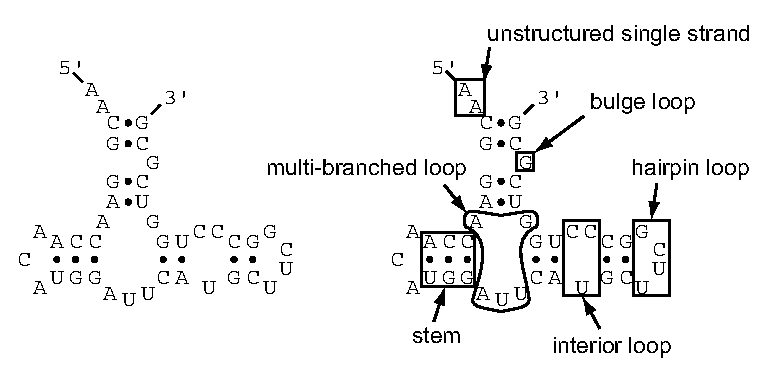
\includegraphics[scale=0.8]{figures/rna_elements}
\end{center}
\begin{center}
\begin{BVerbatim}
  ::((((,<<<___>>>,,,<<-<<____>>-->>,))-))
  AACGGAACCAACAUGGAUUCAUGCUUCGGCCCUGGUCGCG
\end{BVerbatim}
\end{center}

\subsection{Full (output) WUSS notation}

In detail, symbols used by WUSS notation in \emph{output} structure
annotation strings are as follows:

\begin{sreitems}{\textbf{Bulge, interior loops}}
\item[\textbf{Base pairs}]
  Base pairs are annotated by nested matching pairs of symbols
  \verb+<>+, \verb+()+, \verb+[]+, or \verb+{}+.
  The different symbols indicate the ``depth'' of the
  helix in the RNA structure as follows:
  \verb+<>+ are used for simple terminal stems;
  \verb+()+ are used for ``internal'' helices enclosing a multifurcation of
  all terminal stems; \verb+[]+ are used for internal helices
  enclosing a multifurcation that includes at least one annotated
  \verb+()+ stem already; and \verb+{}+ are used for all internal
  helices enclosing deeper multifurcations.

\item[\textbf{Hairpin loops}]
  Hairpin loop residues are indicated by underscores, \verb+_+.
  Simple stem loops stand out as, e.g.\ \verb+<<<<____>>>>+.

\item[\textbf{Bulge, interior loops}]
  Bulge and interior loop residues are indicated by dashes, \verb+-+.

\item[\textbf{Multifurcation loops}]
  Multifurcation loop residues are indicated by commas, \verb+,+.
  The mnemonic is ``stem 1, stem2'', e.g.\ \verb+<<<___>>>,,<<<___>>>+.

\item[\textbf{External residues}]
  Unstructured single stranded residues completely outside the
  structure (unenclosed by any base pairs) are annotated by
  colons, \verb+:+.

\item[\textbf{Insertions}]
  Insertions relative to a known structure are indicated by periods,
  \verb+.+. Regions where local structural alignment was invoked,
  leaving regions of both target and query sequence unaligned,
  are indicated by tildes, \verb+~+. These symbols only appear in
  alignments of a known (query) structure annotation to a target
  sequence of unknown structure.

\item[\textbf{Pseudoknots}]
  WUSS notation allows pseudoknots to be annotated as pairs of
  upper case/lower case letters: for example,
  \verb+<<<<_AAAA____>>>>aaaa+ annotates a simple pseudoknot;
  additional pseudoknotted stems could be annotated by \verb+Bb+,
  \verb+Cc+, etc. 

  This is not a fully general notation. It is possible to come up with
  pseudoknotted structures that could not be represented with 26
  levels of nesting ($>$26th order pseudoknot, in the sense of
  \citep{RivasEddy99}). However, it is unlikely you will ever see one
  in nature. I believe the highest order pseudoknot known is the S1
  (alpha operon) pseudoknot, which is 3rd order.
\end{sreitems}

An example of WUSS notation for a complicated structure
(\emph{E. coli} RNase P) is shown in Figure~\ref{fig:RNaseP}.  An
example of WUSS notation for a local alignment of \emph{B. subtilis}
RNase P to \emph{E. coli} RNase P, illustrating the use of local
alignment annotation symbols, is in Figure~\ref{fig:bsu-alignment}.

\begin{figure}[tp]
\begin{center}
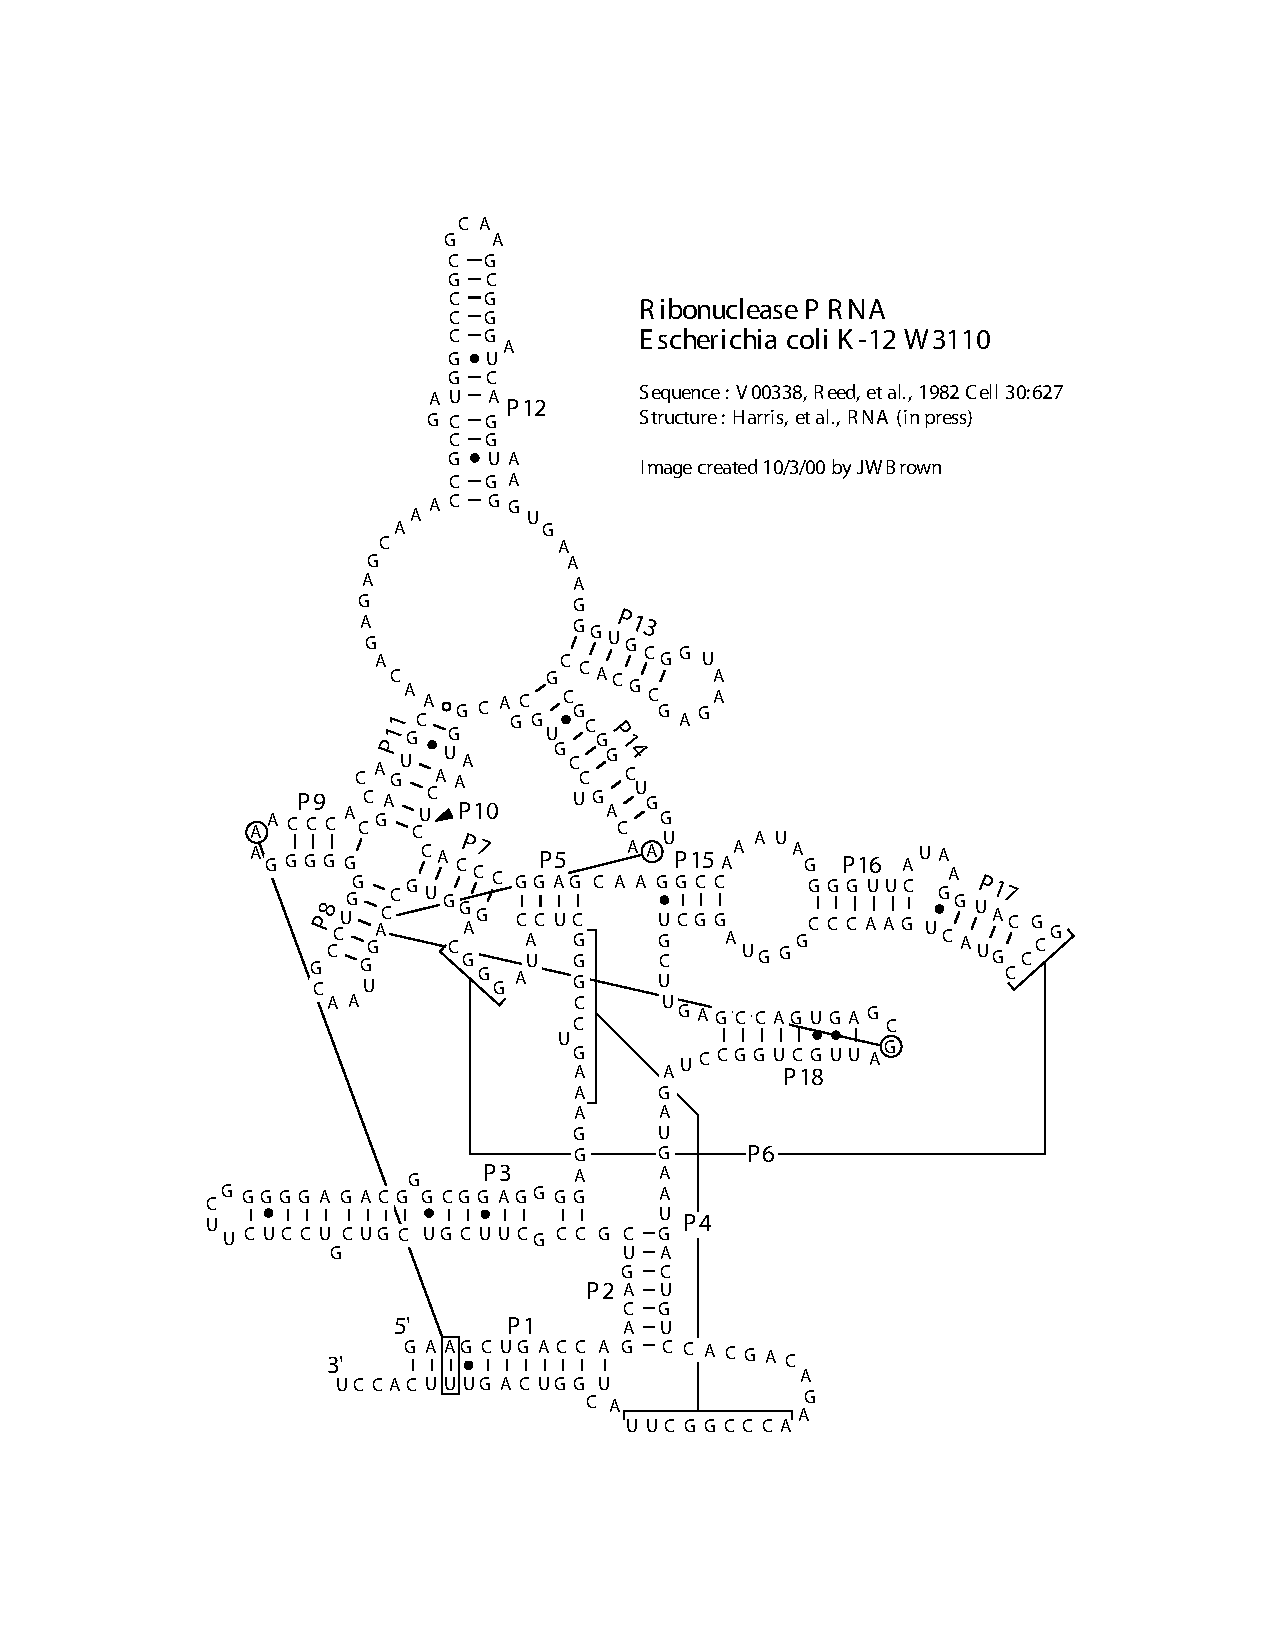
\includegraphics[scale=0.6]{figures/rnaseP-ecoli}
\end{center}
\begin{center}
{\scriptsize
\begin{BVerbatim}
           {{{{{{{{{{{{{{{{{{,<<<<<<<<<<<<<-<<<<<____>>>>>>>>>->>>>>>>>
         1 GAAGCUGACCAGACAGUCGCCGCUUCGUCGUCGUCCUCUUCGGGGGAGACGGGCGGAGGG 60

           >,,,,AAA-AAAAA[[[[---BBBB-[[[[[<<<<<_____>>>>><<<<____>>>->(
        61 GAGGAAAGUCCGGGCUCCAUAGGGCAGGGUGCCAGGUAACGCCUGGGGGGGAAACCCACG 120

           (---(((((,,,,,,,,,,,,<<<<<--<<<<<<<<____>>>>>->>>>>>-->>,,,,
       121 ACCAGUGCAACAGAGAGCAAACCGCCGAUGGCCCGCGCAAGCGGGAUCAGGUAAGGGUGA 180

           ,,,<<<<<<_______>>>>>><<<<<<<<<____>>>->>>>>->,,)))--))))]]]
       181 AAGGGUGCGGUAAGAGCGCACCGCGCGGCUGGUAACAGUCCGUGGCACGGUAAACUCCAC 240

           ]]]]]],,,<<<<------<<<<<<----<<<<<_bbbb>>>>>>>>>>>----->>>>,
       241 CCGGAGCAAGGCCAAAUAGGGGUUCAUAAGGUACGGCCCGUACUGAACCCGGGUAGGCUG 300

           ,,,,,<<<<<<<<____>>>>>>>>,,,,,,,,,,}}}}}}}----------aaaaaaaa
       301 CUUGAGCCAGUGAGCGAUUGCUGGCCUAGAUGAAUGACUGUCCACGACAGAACCCGGCUU 360

           -}-}}}}}}}}}}::::
       361 AUCGGUCAGUUUCACCU 377
\end{BVerbatim}
}
\end{center}
\caption{\small \textbf{Example of WUSS notation.} Top: Secondary
structure of \emph{E. coli} RNase P, from Jim Brown's RNase P database
\citep{Brown99}. Bottom: WUSS notation for the same structure,
annotating the \emph{E. coli} RNase P sequence. Note that the P4 and P6
pseudoknots are annotated, as A's and B's.}
\label{fig:RNaseP}
\end{figure}

\begin{figure}[tp]
\begin{center}
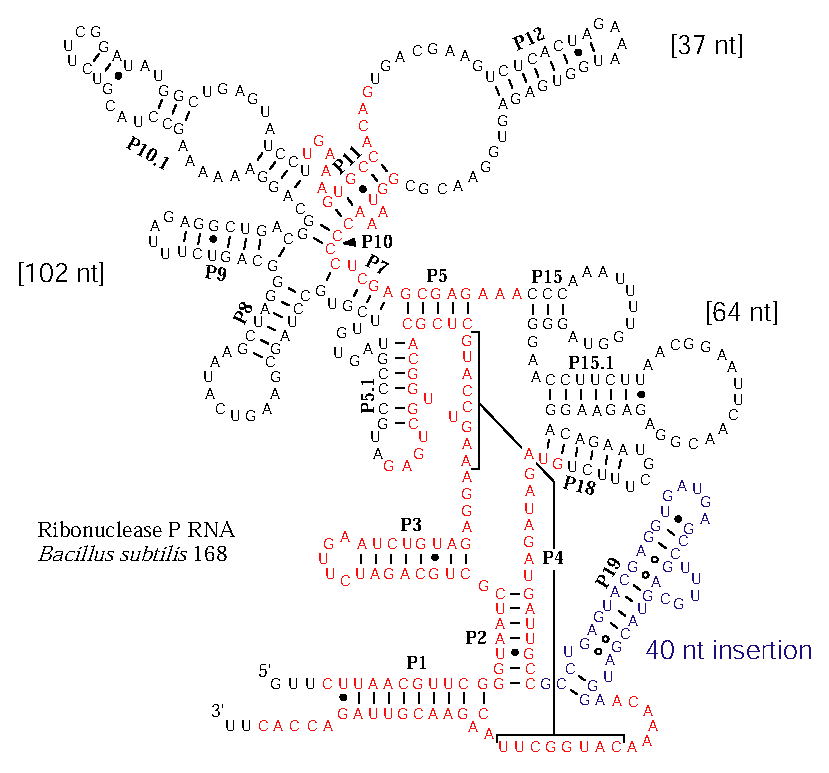
\includegraphics[scale=0.6]{figures/rnaseP-bsu-alignment}
\end{center}
\begin{center}
{\scriptsize
\begin{BVerbatim}
hit 0   :      4    399    52.56 bits
           {{{{{{{{{{{{{{{{{{,<<<<<<<<<<<<<-<<<<<____>>>>>>>>>->>>>>>>>
         1 ggAGuggGgcaGgCaguCGCugcuucggccuuGuucaguuaacugaaaaggAccgaagga 60
           +: :::G::C:GG:A:UCGCU+C::::            U+            ::::G+A
         4 CUUAACGUUCGGGUAAUCGCUGCAGAUC-----------UUG----------AAUCUGUA 42

           >,,,,,,,,,,,,,[[[.[--------[[[[[~~~~~~~((---(((((,,,,~~~~~~)
        61 GAGGAAAGUCCGGGCUC.CACAGGGCAgGGUG*[ 29]*GGAAAGUGCCACAG*[96]*G 229
           GAGGAAAGUCC  GCUC C  A GG   :G G       :GAAAGUGCCACAG      G
        43 GAGGAAAGUCCAUGCUCgC--ACGGUGCUGAG*[102]*UGAAAGUGCCACAG*[37]*G 226

           ))--))))]]]]]].]]],,,~~~~~~,,,,,,,,,,}}}}}}}--..............
       230 GUAAACCCCACCcG.GAGCAA*[77]*CuAGAUGAAUGacuGcCCA.............. 344
           GUAAACC:C C: G GAG AA       UAGAU++AUGA:U:CC
       227 GUAAACCCCUCGAGcGAGAAA*[64]*GUAGAUAGAUGAUUGCC--gccugaguacgagg 342

           ..........................-----------------}-}}}}}}}}}}::::
       345 ..........................CGACAGAACCCGGCUUAuagcCccaCUccucuu 377
                                       ACA AAC  GGCUUA:AG::C::: :+ C
       343 ugaugagccguuugcaguacgaugga--ACAAAACAUGGCUUACAGAACGUUAGACCAC 399
\end{BVerbatim}
}
\end{center}
\caption{\small \textbf{Local alignment annotation example.} Top:
Secondary structure of \emph{B. subtilis} RNase P, from Jim Brown's
RNase P database \citep{Brown99}. Residues in red are those that
Infernal aligns to a CM of \emph{E. coli} type RNase
P's. The local structural alignment is in four pieces; three regions
of the structure (102, 37, and 64 nt long) are skipped over. One
additional stem is treated as a 40 nt insertion. Bottom: the
Infernal output, showing the \emph{E. coli} query structure
aligned to the \emph{B. subtilis} sequence.}
\label{fig:bsu-alignment}
\end{figure}

\subsection{Shorthand (input) WUSS notation}

While WUSS notation makes it easier to visually interpret Infernal
\emph{output} structural annotation, it would be painful to require
people to \emph{input} all structures in full WUSS notation. Therefore
when software like Infernal reads input secondary structure
annotation, it also allows simpler rules:

\begin{sreitems}{\textbf{Single stranded residues}}
\item [\textbf{Base pairs}]
  Any matching nested pair of \verb+()+, \verb+()+, \verb+[]+, \verb+{}+
  symbols indicates a base pair; the exact choice of symbol has no
  meaning, so long as the left and right partners match up.
  Similarly, pseudoknotted pairs can also be annotated by matching nested
  pairs of any alphabet character, such as \verb+Aa+, \verb+Bb+, etc.

\item [\textbf{Single stranded residues}]
  All other symbols \verb+_-,:.~+
  indicate single stranded residues.
  The choice of symbol has no special meaning.
  Annotated pseudoknots (nested matched pairs of upper/lower case
  alphabetic characters) are also interpreted as single
  stranded residues in Infernal input.
\end{sreitems}

Thus, for instance, \verb+<<<<....>>>>+ and \verb+((((____))))+ and
\verb+<(<(._._)>)>+ all indicate a four base stem with a four base
loop (the last example is legal but weird).

Remember that the key property of canonical (nonpseudoknotted) RNA
secondary structure is that the pairs are \emph{nested}.
\verb+((<<....))>>+ is not a legal annotation string: the pair symbols
don't match up properly. 

Because many other RNA secondary structure analysis programs use a
simple bracket notation for annotating structure, the ability to input
the simple format makes it easier to use data generated by other RNA
software packages. Conversely, converting output WUSS notation to
simple bracket notation is a matter of a simple Perl or sed script,
substituting the symbols appropriately.


\newpage
\newcommand{\bibfont}{\footnotesize}
\bibliographystyle{apalike}
\bibliography{master,lab,books}

\end{document}

